\documentclass[11pt,oneside]{article}
\usepackage[margin=1in,headheight=15pt]{geometry}
\usepackage[T1]{fontenc}
\usepackage[utf8]{inputenc}
\usepackage{lmodern}
\usepackage{microtype}
\usepackage{amsmath,amssymb,amsthm,mathtools}
\usepackage{booktabs,longtable,array,tabularx}
\usepackage{enumitem}
\usepackage{xcolor}
\usepackage{listings}
\usepackage{fancyhdr}
\usepackage{hyperref}
\usepackage[nameinlink,noabbrev]{cleveref}
\usepackage{tikz}
\usetikzlibrary{arrows.meta,positioning,fit,calc}

\definecolor{tapirblue}{RGB}{27,73,101}
\definecolor{tapirgreen}{RGB}{35,110,87}
\definecolor{tapirgray}{RGB}{245,247,249}
\definecolor{tapirred}{RGB}{150,45,45}
\hypersetup{colorlinks=true,linkcolor=tapirblue,citecolor=tapirgreen,urlcolor=tapirblue,
  pdftitle={TAPIR-iPRA: A Typed Proof-Plan Compiler for Finitary Mathematics},
  pdfauthor={OpenAI research assistant},
  pdfsubject={Intuitionistic primitive recursive arithmetic and Lean formalization}}
\pagestyle{fancy}
\fancyhf{}
\fancyhead[L]{\small TAPIR-iPRA}
\fancyhead[R]{\small Typed proof-plan compilation}
\fancyfoot[C]{\thepage}
\setlength{\parindent}{0pt}
\setlength{\parskip}{0.55em}
\setlist{nosep,leftmargin=2em}
\setcounter{tocdepth}{2}
\setcounter{secnumdepth}{3}

\newtheorem{theorem}{Theorem}[section]
\newtheorem{lemma}[theorem]{Lemma}
\newtheorem{proposition}[theorem]{Proposition}
\newtheorem{corollary}[theorem]{Corollary}
\newtheorem{definition}[theorem]{Definition}
\newtheorem{remark}[theorem]{Remark}
\newtheorem{example}[theorem]{Example}
\newtheorem{obstruction}[theorem]{Obstruction}

\newcommand{\iPRA}{\mathrm{iPRA}}
\newcommand{\PRAAx}{\mathsf{PRAAx}}
\newcommand{\Prf}{\mathsf{Prf}}
\newcommand{\PTm}{\mathsf{PTm}}
\newcommand{\PR}{\mathsf{PR}}
\newcommand{\Fm}{\mathsf{Fm}}
\newcommand{\Plan}{\mathsf{Plan}}
\newcommand{\TAPIR}{\textsc{Tapir}}
\newcommand{\seq}[3]{#1\;\vdash_{#2}\;#3}
\newcommand{\obj}[2]{#1\;\vdash_{\PRAAx}\;#2}
\newcommand{\Nat}{\mathbb N}
\newcommand{\Bool}{\mathbb B}
\newcommand{\angles}[1]{\langle #1\rangle}
\newcommand{\code}[1]{\nolinkurl{#1}}
\newcommand{\resid}{\mathcal R}
\newcommand{\outputs}{\mathcal O}
\newcommand{\TODO}{\textcolor{tapirred}{\textbf{Formalization milestone}}}
\newcolumntype{P}[1]{>{\raggedright\arraybackslash}p{#1}}
\setlength{\emergencystretch}{2em}

\lstdefinelanguage{Lean}{
  morekeywords={inductive,structure,def,theorem,lemma,namespace,end,open,variable,abbrev,
    import,where,by,exact,refine,match,with,if,then,else,let,in,forall,exists,fun,Type,Prop},
  sensitive=true,
  morecomment=[l]{--},
  morecomment=[s]{/-}{-/},
  morestring=[b]"
}
\lstset{basicstyle=\ttfamily\small,breaklines=true,columns=fullflexible,
  frame=single,backgroundcolor=\color{tapirgray},rulecolor=\color{tapirblue!35},
  xleftmargin=0.5em,xrightmargin=0.5em,aboveskip=0.7em,belowskip=0.7em,
  showstringspaces=false}

\begin{document}
\pagenumbering{gobble}
\begin{titlepage}
\centering
\vspace*{1.2cm}
{\Huge\bfseries\color{tapirblue} TAPIR-iPRA\par}
\vspace{0.35cm}
{\LARGE A Typed Proof-Plan Compiler for Theorem-Specialized Mathematics in Intuitionistic Primitive Recursive Arithmetic\par}
\vspace{0.9cm}
{\large Human proofs, a Lean integration design, executable reference algorithms, and a difficulty audit\par}
\vfill
\begin{minipage}{0.88\textwidth}
\colorbox{tapirgray}{\parbox{0.94\textwidth}{
\textbf{Repository baseline.} VladimirReshetnikov/ProveIt, branch \code{main}, commit
\code{58627ed89814ba122e1f0f012f1aba103cda267b}, inspected 16 November 2026.

\textbf{Verification status.} This report proves the generic mathematics on paper and supplies two
small, no-placeholder Lean source candidates for the typed kernel and sequential schedule compiler.
No Lean executable was available in the artifact runtime, so no new declaration is claimed to have
been elaborated or kernel-checked. Existing ProveIt declarations cited as checked are inherited
upstream results. Python tests validate only the finite host algorithms; they are not an iPRA proof
checker.
}}
\end{minipage}
\vfill
{\large 16 November 2026\par}
\end{titlepage}
\pagenumbering{roman}

\begin{abstract}
The ProveIt iPRA repository now contains a checked object calculus, a substantial library of
ordinary derivations, and more than one hundred mathematical proof packets.  The packets repeatedly
exhibit the same mismatch: finite search, exact arithmetic, trace checking, and certificate
verification are easy to describe at the host level, but the final claim is often not a term of the
canonical judgment \(\Prf\,\PRAAx\,\Gamma\,\varphi\).  Several prior frameworks solve the semantic
part of the problem, yet leave a generic last-mile compiler as a blueprint.

This report proposes \TAPIR-iPRA (\emph{Typed Arithmetic Proof Intermediate Representation}).  Its
central idea is deliberately modest: do not internalize a universal syntax interpreter inside iPRA.
Instead, specialize every mathematical construction at Lean elaboration time to concrete \(\PR\),
\(\PTm\), and \(\Fm\) expressions, and represent the resulting argument by an indexed proof plan
whose type already states its object-theory endpoint.  A total interpreter from plans to
\(\Prf\,\PRAAx\) is then a structural recursion using only checked constructors and checked library
lemmas.  An untrusted host generator may build plans, but it cannot manufacture a theorem because
Lean must accept the generated term.

The second ingredient is a typed sequential schedule.  A new node is allowed to use earlier outputs
and a fixed list of residual producer hypotheses.  Simultaneous cut discharges all earlier outputs,
so induction on the schedule produces a proof of every node from the residuals alone.  Consequently,
a finite contract graph compiles to an ordinary sequent
\[
  B_1,\ldots,B_r,\Gamma\;\vdash_{\PRAAx}\;\Phi,
\]
with no hidden oracle.  Supplying object proofs of the \(B_i\) closes the theorem; otherwise the
conditional endpoint precisely records what mathematics is still missing.

The report integrates certificate escape analysis, bounded least-witness extraction, compositional
bounded reflection, clocked traces, quantitative names, stable observations, and height-bounded
enumeration.  It resolves several difficulties that older packets had left open by reusing current
checked modules: \code{Prf.subst}, \code{Prf.weaken}, \code{Prf.trans}, quantifier-free induction,
least bounded search, bounded universal and existential reflection, pairing, and measure-decreasing
termination.  It does not claim ineffective height bounds, convergence moduli, separation constants,
or uniform generator algorithms.  Those remain explicit producer boundaries rather than being
smuggled into a purported compiler.

The archive contains the complete \LaTeX{} source and PDF, Lean-oriented modules and a
formalization plan, an executable reference implementation of graph slicing, schedule validation,
escape analysis, finite strategy synthesis, demand closure, and traces, together with tests and
machine-readable metadata.
\end{abstract}

\section*{Main contribution at a glance}
\addcontentsline{toc}{section}{Main contribution at a glance}

\begin{center}
\resizebox{0.97\textwidth}{!}{%
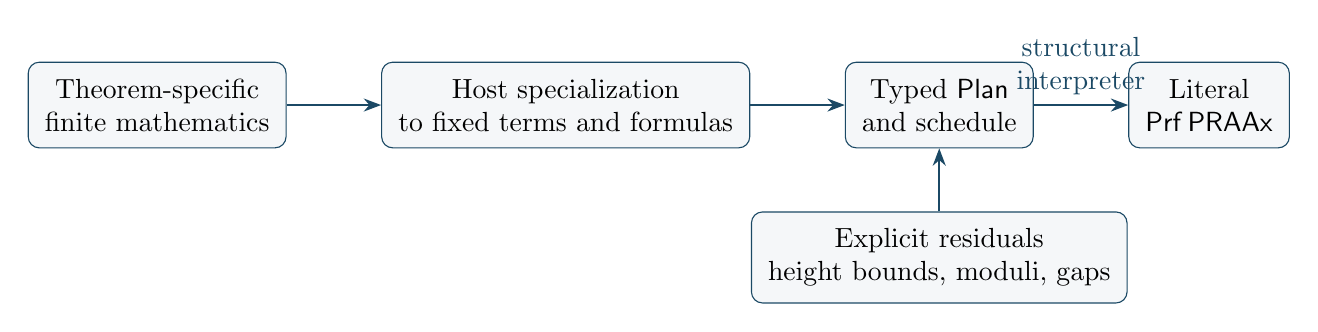
\begin{tikzpicture}[
  node distance=8mm and 12mm,
  box/.style={draw=tapirblue,rounded corners,fill=tapirgray,align=center,inner sep=6pt},
  arr/.style={-{Stealth[length=2.2mm]},thick,tapirblue}]
\node[box] (math) {Theorem-specific\\finite mathematics};
\node[box,right=of math] (specialize) {Host specialization\\to fixed terms and formulas};
\node[box,right=of specialize] (plan) {Typed \(\Plan\)\\and schedule};
\node[box,right=of plan] (prf) {Literal\\\(\Prf\,\PRAAx\)};
\draw[arr] (math) -- (specialize);
\draw[arr] (specialize) -- (plan);
\draw[arr] (plan) -- node[above,align=center]{structural\\interpreter} (prf);
\node[box,below=of plan] (res) {Explicit residuals\\height bounds, moduli, gaps};
\draw[arr] (res) -- (plan);
\end{tikzpicture}%
}
\end{center}

The framework is not a stronger theory.  It is a disciplined way to obtain ordinary iPRA
proofs from the finite constructions that iPRA can actually express, while making every stronger
input visible in the context.

\tableofcontents
\clearpage
\pagenumbering{arabic}
\section{Repository baseline and diagnosis}\label{sec:baseline}

\subsection{The checked core already available}

The pinned repository has three layers that must be kept distinct.

\begin{enumerate}
\item \textbf{The object calculus.}  \code{ConciseIPRA} defines primitive-recursive symbols
\(\PR k\), terms \(\PTm n\), formulas \(\Fm\,\PTm\,n\), the axiom family \(\PRAAx\), and the
intuitionistic natural-deduction judgment
\[
   \Prf\,\PRAAx\,\Gamma\,\varphi,
   \qquad\text{written}\qquad \Gamma\vdash_{\PRAAx}\varphi.
\]
The calculus has scoped substitution, weakening, simultaneous cut, first-order quantifiers,
equality substitution, and quantifier-free induction.

\item \textbf{Checked mathematical derivations.}  \code{IPRADerivations} gives object-level
proofs for arithmetic operations, order, bounded sums and products, pairing, search, finite
combinatorics, termination, and many theorem-specific developments.  In particular, the current
\code{Core/Search.lean} proves the least-search specification, while
\code{Foundations/BoundedReflection.lean} proves bounded universal and existential reflection and a
least-witness theorem.  These are not mere semantic lemmas about Lean functions: their conclusions
are sequents in \(\Prf\,\PRAAx\).

\item \textbf{Research packets.}  The catalogue under \code{docs/proofs} contains broad analyses,
formalization outlines, and executable finite checkers.  Their scientific value is substantial, but
most packets explicitly do not claim a constructed proof of their main theorem in the object
calculus.  Framework packets have converged on finite certificates, explicit moduli, stable
observers, residual producer hypotheses, and proof-graph composition, but many of their generic Lean
modules remain unelaborated blueprints.
\end{enumerate}

The correct goal is therefore not to invent another semantics for iPRA.  It is to connect finite
mathematical arguments to the already checked endpoint with the least possible new trusted code.

\subsection{What the repository has learned}

Across algebra, analysis, number theory, geometry, probability, and foundations, the same lessons
recur.

\paragraph{Fixed finite questions are the natural unit.}
An iPRA theorem about an analytic function is not best represented by a completed real-number
universe.  It is represented by a primitive-recursive approximation program together with a theorem
that answers every fixed precision request.  Likewise, a compactness argument is represented by an
explicit finite cover or net, an algebraic classification by a finite list plus completeness proof,
and a computation by a clocked trace plus an invariant.

\paragraph{Verification is easier than production.}
Given a candidate factorization, path, cover, height bound, separation gap, or convergence modulus,
its finite correctness is often primitive recursive and amenable to bounded reflection.  Producing
such data uniformly can be much harder or impossible at the intended strength.  The framework must
therefore distinguish a producer from its verifier.

\paragraph{Noncanonical witnesses should usually be sealed.}
A proof may need a root, chart, basis, triangulation, or local branch without needing to expose which
one was selected.  Searching for a canonical code adds an unnecessary bound and can create a false
uniformity claim.  Ordinary existential elimination is the correct rule when only a
certificate-independent conclusion escapes.

\paragraph{Approximation is not equality.}
A small-diameter cloud of candidates supports stable numerical observations.  It does not by itself
supply an exact label.  Exact branch recovery requires an additional separation gap.  The theorem
statement must preserve that distinction.

\paragraph{Quantifier-free induction is sufficient when the state is designed correctly.}
The induction formula should be a finite arithmetic invariant of a primitive-recursive state.  All
precision parameters, resource budgets, and demanded observations are frozen before induction or
stored as state fields.  Rich mathematical conclusions are extracted after the trace theorem.

\subsection{The remaining bottleneck}

Earlier frameworks frequently reach a statement of the following shape at the meta level:

\begin{quote}
A bounded checker accepted a certificate; every accepted certificate has a valid trace; the final
trace state satisfies the desired finite observation; therefore the theorem follows in iPRA.
\end{quote}

Three gaps can hide inside that sentence.

\begin{enumerate}[label=\textbf{G\arabic*.}]
\item A Python or Lean Boolean computation has been mistaken for an object proof of its correctness.
\item A host-level graph has been declared compositional without producing the sequence of
\code{Prf.trans}, \code{Prf.subst}, binder shifts, and quantifier rules required by the scoped
calculus.
\item A deep producer---for example a general height cutoff---has been folded into the word
``certificate'' even though only verification is primitive recursive.
\end{enumerate}

\TAPIR{} addresses G1 and G2 by making the intermediate language intrinsically indexed by the
object sequent and by compiling a schedule through the checked structural operations.  It addresses
G3 by residualization: producer statements remain formulas in the antecedent until an actual object
proof discharges them.

\subsection{Why a universal internal proof checker is the wrong target}

One tempting response is to encode arbitrary proof graphs, terms, formulas, and evaluators by
natural numbers and prove a universal soundness theorem inside iPRA.  That direction has three costs.

First, there is no total primitive-recursive universal evaluator for all primitive-recursive
programs.  A fixed bounded interpreter can be built for a fixed language and fuel, but a silent
universal evaluator assumption is unsound.  Second, the repository already has a trusted Lean
representation of syntax and derivations; re-encoding it internally duplicates binder and
substitution work.  Third, most applications are theorem-specific: the graph, arithmetic symbols,
and requested precision are known before elaboration.

The proposed compiler therefore uses \emph{staging}.  Host computation specializes a fixed finite
argument to concrete syntax.  The generated object proof is checked by Lean.  Soundness is obtained
from the type and the structural interpreter, not from trusting the host generator.

\subsection{Scope of the claimed resolution}

This report claims a resolution of the following framework-level problems:

\begin{itemize}
\item a small typed IR whose interpreter returns literal \(\Prf\,\PRAAx\) terms;
\item a schedule theorem that composes finite acyclic proof graphs by simultaneous cut;
\item a precise rule for local, observed, and publicly named certificates;
\item a compositional interface for bounded reflection using the checked least-search backend;
\item a reusable trace pattern compatible with quantifier-free induction;
\item a residual theorem normal form for all unresolved producers.
\end{itemize}

It does not claim to solve general effective Faltings, Siegel, Mordell--Weil, ineffective analytic
constants, or missing separation estimates.  It shows exactly how such an input would be consumed
and exactly what theorem is available without it.

\section{Design principles}\label{sec:design}

\subsection{The endpoint is part of every type}

A framework object is acceptable only when its type records an actual object-theory judgment.  We
write
\[
  \mathsf{Deriv}_n(\Gamma,\varphi)
  := \Prf\,\PRAAx\,\Gamma\,\varphi.
\]
A host-level proposition such as ``the checker returned true'' is not interchangeable with
\(\mathsf{Deriv}_n(\Gamma,\varphi)\).  The bridge between them must itself be an object derivation,
typically a reflection theorem specialized to the checker.

This principle prevents a common ambiguity.  A Lean theorem about the standard natural numbers may
be mathematically correct while proving nothing about derivability in iPRA.  In \TAPIR{}, semantic
lemmas are useful for testing, but reusable proof nodes must return \(\mathsf{Deriv}\) or a typed plan
that structurally compiles to it.

\subsection{Theorem specialization, not universal evaluation}

Suppose a mathematical proof uses a fixed transition program \(s\), a fixed checker \(v\), and a
fixed formula \(\Phi\).  The host compiler constructs concrete objects
\[
  s^{\sharp}:\PR k,\qquad v^{\sharp}:\PTm n,\qquad \Phi^{\sharp}:\Fm\,\PTm\,n.
\]
It then emits a plan assembled from library theorems specialized by
\code{Prf.subst}.  No object-level function receives the code of an arbitrary program and evaluates
it.  Meta-level recursion on the syntax tree is permitted because it produces a finite Lean term;
the kernel verifies the result.

This is analogous to proof-producing compilation.  The compiler is not trusted for soundness.  A
bug can make it fail, produce an ill-typed term, or prove a weaker theorem, but it cannot cause Lean
to accept an invalid \(\Prf\) value without a defect in the checked kernel or imported axioms.

\subsection{A small macro IR is preferable to a second logic}

The IR should not duplicate natural deduction.  Its constructors are macros for operations already
available in the checked calculus:

\begin{center}
\begin{tabular}{lll}
\toprule
IR operation & Checked implementation & Mathematical role \\
\midrule
embed & existing \(\Prf\) term & reuse arithmetic/domain lemma \\
specialize & \code{Prf.subst} & instantiate a theorem schema \\
weaken & \code{Prf.weaken} & align contexts \\
cut & \code{Prf.trans} & compose nodes / discharge outputs \\
seal & \code{Prf.exE} & eliminate proof-local certificate \\
name & checked bounded choice & expose least bounded witness \\
loop & \code{PRA.qfInd} & verify a clocked invariant \\
close & a second \code{Prf.trans} & discharge residual producers \\
\bottomrule
\end{tabular}
\end{center}

The IR is useful because it gives a uniform target for generators and enforces scoping, but its
interpreter is transparent and small.

\subsection{Residual hypotheses are first-class}

Let \(B_1,\ldots,B_r\) be producer statements such as:

\begin{itemize}
\item every solution has height at most \(H(q)\);
\item a rational approximation has an error below \(2^{-p}\);
\item a branch is separated from all competitors by \(\delta\);
\item a finite cover is complete;
\item a constant \(C\) satisfies the explicit inequalities needed by the proof.
\end{itemize}

The compiler is required to produce
\[
 B_1,\ldots,B_r,\Gamma\vdash_{\PRAAx}\Phi.
\]
It is forbidden to replace an unavailable \(B_i\) by a host assertion.  If a later development
proves \(\Delta\vdash B_i\) for every residual, simultaneous cut immediately produces
\(\Delta,\Gamma\vdash\Phi\).  Thus residualization is not an admission of failure; it is a stable
modular interface.

\subsection{Certificate escape analysis}

Every existential datum is assigned one of three modes.

\begin{description}
\item[Local.] The witness occurs only inside the proof.  It is introduced existentially and sealed
by \code{Prf.exE}.  No code bound is needed merely to eliminate it.

\item[Observed.] The witness is noncanonical, but the public theorem mentions an invariant or stable
observation.  The local proof establishes that every valid witness gives the same observation, or
observations within a specified diameter.  The witness is then sealed.

\item[Named.] The public result explicitly returns a code, a least witness, a branch label, or a
function of the witness.  A complete bounded search space and a decidable verifier are required.
The checked bounded-choice theorem may then expose a primitive-recursive least witness.
\end{description}

This analysis prevents finite existence from silently becoming a uniform choice function.

\subsection{Static resources and dynamic state}

A proof generator first performs a reverse pass that computes all precisions, horizons, finite-set
sizes, and observation demands.  These values are fixed terms by the time object induction begins.
The forward object proof uses a single primitive-recursive state and a quantifier-free invariant.
If a resource must change during a run, it is represented as a state field and its update is included
in the step equation.

The point is logical, not merely algorithmic.  An induction schema applies to one fixed formula.  A
proof that informally changes its precision parameter at every step must be rewritten so that the
precision is a parameter or a component of the state.

\subsection{A trust budget}

The proposed trust boundary is:

\begin{enumerate}
\item Lean's kernel and the imported checked ProveIt definitions;
\item the concrete \(\Prf\) term produced by the plan interpreter;
\item no trust in Python tests, JSON certificates, numerical experiments, or host graph generators.
\end{enumerate}

Executable artifacts remain valuable: they detect malformed schedules, arithmetic mistakes, and
resource bugs before formalization.  Their role is regression testing and certificate production,
not logical justification.

\section{The typed arithmetic proof IR}\label{sec:typed-ir}

\subsection{Judgments and notation}

Fix a number \(n\) of free variables.  A context is a list
\(\Gamma:\mathsf{List}(\Fm\,\PTm\,n)\), and a conclusion is
\(\varphi:\Fm\,\PTm\,n\).  The canonical object judgment is
\[
  \Gamma\vdash_{\PRAAx}\varphi.
\]
All substitutions are simultaneous and scoped.  If
\(\sigma:\mathrm{Fin}(n)\to\PTm\,m\), then
\(\Gamma[\sigma]\) denotes the pointwise substitution in the context and
\(\varphi[\sigma]\) the substituted conclusion.

\begin{definition}[Typed proof plan]
A proof plan \(\Plan(\Gamma,\varphi)\) is an indexed host datatype generated by the following
constructors.

\begin{enumerate}
\item \(\mathsf{prf}(d)\), where \(d:\Gamma\vdash_{\PRAAx}\varphi\).
\item \(\mathsf{weaken}(p,s)\), where \(p:\Plan(\Gamma,\varphi)\) and
      \(s:\Gamma\subseteq\Delta\); its type is \(\Plan(\Delta,\varphi)\).
\item \(\mathsf{subst}(p,\sigma)\), of type
      \(\Plan(\Gamma[\sigma],\varphi[\sigma])\).
\item \(\mathsf{cut}(p,e)\), where \(p:\Plan(\Gamma,\varphi)\) and
      \(e\) assigns to every \(\psi\in\Gamma\) a plan \(e_\psi:\Plan(\Delta,\psi)\);
      its type is \(\Plan(\Delta,\varphi)\).
\item The usual introduction and elimination macros for conjunction, disjunction, implication,
      universal quantification, and existential quantification, with exactly the scoped context
      changes of \(\Prf\).
\item \(\mathsf{qfInd}(Q,p_0,p_S)\), where \(Q\) is quantifier free,
      \(p_0\) proves the zero instance, and \(p_S\) proves the successor instance from the induction
      hypothesis.  Its conclusion is \(\forall x\,Q(x)\).
\end{enumerate}
\end{definition}

The actual Lean candidate in the archive includes the natural-deduction constructors rather than
encoding them through a generic \code{prf} node.  This makes generated plans readable and allows a
future printer or optimizer to see their structure.  Nevertheless, the IR remains a macro layer:
there is no new axiom and no independent notion of validity.

\subsection{The interpreter}

Define \(\mathsf{run}:\Plan(\Gamma,\varphi)\to
(\Gamma\vdash_{\PRAAx}\varphi)\) recursively:

\begin{align*}
\mathsf{run}(\mathsf{prf}(d))&=d,\\
\mathsf{run}(\mathsf{weaken}(p,s))&=\mathsf{Prf.weaken}(\mathsf{run}(p),s),\\
\mathsf{run}(\mathsf{subst}(p,\sigma))&=\mathsf{Prf.subst}(\mathsf{run}(p),\sigma),\\
\mathsf{run}(\mathsf{cut}(p,e))&=\mathsf{Prf.trans}
   (\mathsf{run}(p),\psi\mapsto\mathsf{run}(e_\psi)),
\end{align*}
and similarly for the logical rules.  The induction node is interpreted by
\code{PRA.qfInd}.

\begin{theorem}[Plan soundness]\label{thm:plan-soundness}
For all \(n,\Gamma,\varphi\), every \(p:\Plan(\Gamma,\varphi)\) determines an ordinary object
proof \(\mathsf{run}(p):\Gamma\vdash_{\PRAAx}\varphi\).
\end{theorem}

\begin{proof}
Proceed by structural induction on \(p\).  The \(\mathsf{prf}\) case returns its stored derivation.
The weakening and substitution cases use the already checked closure theorems for \(\Prf\).  In the
cut case, the induction hypothesis yields a derivation of \(\varphi\) from \(\Gamma\) and, for every
member \(\psi\) of \(\Gamma\), a derivation of \(\psi\) from \(\Delta\).  The checked simultaneous
cut theorem \code{Prf.trans} gives \(\Delta\vdash\varphi\).  Each propositional or quantifier case is
exactly the corresponding constructor of \(\Prf\), so the scoped shifts and binder conditions are
already enforced by the type.  Finally, the induction case has precisely the premises of
\code{PRA.qfInd}: a proof that the formula is quantifier free, a base derivation, and a successor
derivation under the shifted context and induction hypothesis.  Applying that theorem yields the
required universal conclusion.  No semantic interpretation of formulas is used.
\end{proof}

\begin{corollary}[Generator untrustworthiness is harmless]
Suppose a host program attempts to generate a plan of type \(\Plan(\Gamma,\varphi)\).  If it succeeds
and Lean accepts the term, then \(\Gamma\vdash_{\PRAAx}\varphi\).  Soundness does not depend on the
correctness of the host program.
\end{corollary}

\begin{proof}
Apply \cref{thm:plan-soundness}.  A malformed graph, incorrect substitution, or missing premise
prevents construction of the indexed term or causes elaboration to fail.  The host program is not an
axiom and does not appear in the object proof.
\end{proof}

\subsection{Why the IR is not circular}

Because \(\mathsf{prf}\) embeds existing derivations, one might object that the plan merely renames
\(\Prf\).  The point of the IR is not to reduce the logical core.  It gives a stable, typed target for
proof generators and collects the high-level composition patterns that research packets repeatedly
reimplement.  The nontrivial work appears in two places:

\begin{enumerate}
\item checked library nodes that transform finite arithmetic evidence into object derivations; and
\item the schedule compiler of \cref{sec:schedule}, which turns a graph of local derivations into a
      root derivation while respecting contexts and residuals.
\end{enumerate}

A compiler that emitted raw \(\Prf\) terms directly would be equally sound.  The plan layer is an
engineering abstraction that makes scoping, residuals, certificate modes, and optimization explicit.

\subsection{Derived macros}

The following macros are especially useful.

\paragraph{Closed reuse.}
If \(p:\Plan([],\varphi)\), then \(\mathsf{ofNil}(p):\Plan(\Gamma,\varphi)\) is weakening along the
empty subset.  This imports a checked arithmetic theorem under arbitrary hypotheses.

\paragraph{Specialization.}
A theorem with \(k\) free variables can be specialized to arbitrary terms by a substitution vector.
This is the primary mechanism by which one generic domain lemma serves many theorem-specific nodes.

\paragraph{Context alignment.}
Local node contexts are normally subsets of ``earlier outputs plus residuals.''  Weakening aligns a
small natural context with the schedule context; simultaneous cut later removes the extra hypotheses.

\paragraph{Sealing.}
Given a plan for \(\exists c\,C(c)\) and a plan of the public conclusion from \(C(c)\) under the
shifted context, existential elimination gives a plan in which \(c\) cannot occur in the conclusion.
The type enforces non-escape.

\paragraph{Residual closure.}
If \(p:\Plan(\resid++\Gamma,\varphi)\) and every formula in \(\resid\) has a plan from \(\Delta\),
then cut produces \(\Plan(\Delta++\Gamma,\varphi)\), after routine context alignment.  A conditional
research packet can therefore be closed without changing its internal proof graph.

\subsection{Optional native-clause backend}

The repository also contains the checked clause calculus \code{KPrf}, with substitution, cut, and an
export to the native kernel.  A future optimizer may lower long equational fragments of a plan to
\code{KPrf}, share repeated traces there, and export back through the checked equivalence with
ordinary iPRA.  This is an optimization, not a requirement.  The primary endpoint of \TAPIR{} is
always the ordinary \(\Prf\,\PRAAx\) judgment so that applications do not depend on a second public
logic.

\subsection{Lean skeleton}

The essential source is intentionally short:

\begin{lstlisting}[language=Lean]
inductive Plan : {n : Nat} -> List (Fm PTm n) -> Fm PTm n -> Type
  | prf    (h : Gamma |-phi) : Plan Gamma phi
  | weaken (p : Plan Gamma phi) (s : Gamma subset Delta) : Plan Delta phi
  | subst  (p : Plan Gamma phi) (sigma : Fin n -> PTm m) :
      Plan (Gamma.map fun psi => psi.subst sigma) (phi.subst sigma)
  | cut    (p : Plan Gamma phi)
      (s : forall psi, psi in Gamma -> Plan Delta psi) : Plan Delta phi
  | exE    (p : Plan Gamma (Fm.ex theta))
      (q : Plan (theta :: Gamma.map Fm.shift) psi.shift) : Plan Gamma psi
  | qfInd  (hq : theta.QF)
      (p0 : Plan Gamma (theta.subst (Syn.inst zero)))
      (pS : Plan (theta :: Gamma.map Fm.shift)
        (theta.subst (Syn.repl (succ (var 0))))) : Plan Gamma (Fm.all theta)
  -- propositional and remaining quantifier constructors omitted here

def Plan.run : Plan Gamma phi -> (Gamma |-phi)
  | .prf h          => h
  | .weaken p s     => (run p).weaken s
  | .subst p sigma  => (run p).subst sigma
  | .cut p s        => (run p).trans (fun psi h => run (s psi h))
  | .exE p q        => Prf.exE (run p) (run q)
  | .qfInd hq p0 pS => PRA.qfInd _ hq (run p0) (run pS)
  -- remaining cases are direct
\end{lstlisting}

The archive gives the fuller candidate with the actual notation and imports.  It has no
\code{sorry}; however, in the absence of Lean in the runtime, this is a source candidate rather than
a compilation claim.

\section{Sequential schedules and proof-graph compilation}\label{sec:schedule}

\subsection{From DAGs to schedules}

A finite proof graph can be topologically sorted.  Rather than formalizing arbitrary graph theory in
the logical kernel, \TAPIR{} uses a sequential schedule whose order is produced by an untrusted host
pass and verified by its type.

Fix a residual context \(R\).  A schedule records a list \(O\) of already produced formulas, in
reverse chronological order.  It is generated by:

\begin{align*}
  \mathsf{nil}&:\mathsf{Schedule}(R,[]),\\
  \mathsf{cons}(S,p)&:\mathsf{Schedule}(R,\varphi::O),
\end{align*}
where \(S:\mathsf{Schedule}(R,O)\) and the local plan
\[
  p:\Plan(O++R,\varphi)
\]
may use any earlier output and any residual hypothesis.  If a natural local proof uses only a subset
of \(O++R\), it is weakened to this canonical context.

The reverse order is convenient: the newest output is the head, while all of its dependencies are in
the tail.  A DAG with several roots can be represented by adding a final node that conjoins or
otherwise packages the desired outputs.

\subsection{Compilation theorem}

\begin{theorem}[Schedule compilation]\label{thm:schedule-compile}
Let \(S:\mathsf{Schedule}(R,O)\).  For every \(\psi\in O\), there is a plan
\[
  \mathsf{compile}(S,\psi):\Plan(R,\psi).
\]
Consequently, if \(O=\varphi::O'\), the head has a plan from the residuals alone.
\end{theorem}

\begin{proof}
Induct on \(S\).

For the empty schedule there is no \(\psi\in[]\), so the assertion is vacuous.

Suppose \(S=\mathsf{cons}(S_0,p)\), where
\(S_0:\mathsf{Schedule}(R,O_0)\) and
\(p:\Plan(O_0++R,\varphi)\).  Let \(\psi\in\varphi::O_0\).

If \(\psi=\varphi\), apply the cut constructor to \(p\).  Every hypothesis
\(\chi\in O_0++R\) is discharged as follows.  If \(\chi\in O_0\), the induction hypothesis supplies
\(\Plan(R,\chi)\).  If \(\chi\in R\), use the hypothesis plan
\(\mathsf{prf}(\mathsf{Prf.hyp})\).  Simultaneous cut therefore yields
\(\Plan(R,\varphi)\).

If \(\psi\in O_0\), use the induction hypothesis directly.  These cases exhaust membership in the
cons list.
\end{proof}

The proof is constructive and mirrors a short Lean recursion.  It is the last-mile graph compiler
that prior packets often described semantically but did not connect to the ordinary context calculus.

\begin{corollary}[Acyclic contract graph]\label{cor:dag}
Let a finite directed acyclic graph have nodes labeled by formulas.  Suppose every node \(v\) carries
a local plan deriving its label from the labels of its predecessors and residual context \(R\).  Then
every root label is derivable from \(R\) in \(\PRAAx\).
\end{corollary}

\begin{proof}
Choose any topological order and build a schedule.  At each stage, all predecessors are earlier
outputs.  Weaken the local plan from its actual dependency list to the full list of earlier outputs
plus \(R\).  Apply \cref{thm:schedule-compile} to the root node.
\end{proof}

\subsection{Closing residuals}

\begin{theorem}[Residual closure]\label{thm:residual-close}
If \(R\vdash_{\PRAAx}\varphi\) and for every \(B\in R\) one has
\(\Delta\vdash_{\PRAAx}B\), then \(\Delta\vdash_{\PRAAx}\varphi\).
\end{theorem}

\begin{proof}
This is exactly simultaneous cut, \code{Prf.trans}.  No induction on the mathematical proof graph is
needed because the schedule compiler has already reduced the graph to one ordinary derivation from
\(R\).
\end{proof}

A useful consequence is monotonic development.  A packet may initially expose five residuals.  A
later theorem can discharge two of them, producing a stronger packet with three residuals by a
single cut, without regenerating the internal proof.

\subsection{Exactness of the residual list}

The phrase ``exact residuals'' is syntactic, not a claim of logical independence.  The host compiler
performs a backward slice from the selected root, removes unreachable nodes, and takes the union of
external boundaries actually mentioned by the reachable local plans.  The resulting schedule has
that list as its context.  Therefore:

\begin{proposition}[Syntactic residual exactness]\label{prop:residual-exact}
For a sliced schedule generated by the reference algorithm, every formula in the reported residual
list occurs in at least one reachable local context, and no external formula absent from that list is
used by the compiled plan.
\end{proposition}

\begin{proof}
The first assertion follows from how the union is accumulated during the backward traversal; a
boundary is inserted only when a reachable node declares it.  The second follows by induction on the
schedule: each local plan is typed over earlier outputs plus the reported residual context, and the
compiler introduces no new hypotheses.  This does not prove that a residual is mathematically
indispensable; another proof may avoid it.
\end{proof}

\subsection{Dead-code elimination}

Let \(G\) be a finite graph and \(r\) a root.  Define \(\mathrm{reach}(r)\) as the least set containing
\(r\) and every predecessor of a member.  Delete all other nodes before topological sorting.

\begin{lemma}[Backward slicing preserves the root proof]
If every dependency named by a reachable node is retained, deleting unreachable nodes does not
change the local proof of any reachable node and hence does not change the compiled root plan.
\end{lemma}

\begin{proof}
By induction on a topological order of the reachable subgraph.  A reachable node's local plan uses
only declared predecessors and residuals.  Every declared predecessor is reachable by definition,
so its compiled plan remains available.  Unreachable outputs are never selected in the discharge
function used by cut.
\end{proof}

This elementary optimization matters in large packets: it prevents the final object proof from
containing unrelated certificates or producer assumptions.

\subsection{Cycles and demand closure}

The proof schedule itself is acyclic.  A mathematical construction may have cyclic resource
dependencies---for example, a requested precision at one node increases the requirement at another.
Those cycles are resolved in a separate finite host pass.  On a product of finite chains, iterate
\[
 d_{t+1}=d_t\vee F(d_t)
\]
from the least demand.  If \(F\) is monotone, the sequence stabilizes at the least prefixed point;
each strict iteration increases at least one coordinate, so no more than the sum of coordinate
capacities is needed.  The stabilized numerical demand is then frozen and inserted into the acyclic
proof schedule.

If the closure itself is part of the public theorem, a clocked object trace can verify it.  Usually it
is merely a compile-time resource calculation, in which case Lean checks only the specialized proof
that uses the resulting constants.

\subsection{Host algorithm and verification conditions}

The reference compiler performs:

\begin{enumerate}
\item parse nodes, dependencies, conclusions, and residual declarations;
\item reject duplicate identifiers, missing dependencies, and cycles;
\item backward-slice from the selected root;
\item topologically order the slice;
\item compute the residual union and certificate escape modes;
\item emit a schedule description and, eventually, Lean source that constructs the corresponding
      \(\mathsf{Schedule}\) value.
\end{enumerate}

Only the final Lean value matters for soundness.  The Python implementation in the archive tests the
finite algorithms and produces JSON examples, but it is explicitly not a checker for
\(\Prf\,\PRAAx\).

\subsection{Lean form of the schedule theorem}

The index-safe list formulation avoids formula-code equality and arbitrary graph indices:

\begin{lstlisting}[language=Lean]
inductive Schedule {n : Nat} (R : List (Fm PTm n)) :
    List (Fm PTm n) -> Type
  | nil : Schedule R []
  | cons {outs : List (Fm PTm n)} {phi : Fm PTm n}
      (tail : Schedule R outs)
      (local : Plan (outs ++ R) phi) : Schedule R (phi :: outs)

private def dischargeAppend
    (ih : forall psi, psi in outs -> Plan R psi) :
    forall psi, psi in outs ++ R -> Plan R psi := by
  intro psi h
  rcases List.mem_append.mp h with hOut | hR
  case inl => exact ih psi hOut
  case inr => exact Plan.prf (Prf.hyp hR)

def Schedule.proveAll :
    (s : Schedule R outs) -> forall psi, psi in outs -> Plan R psi
  | .nil, _, h => by simp at h
  | .cons tail local, psi, h => by
      rcases List.mem_cons.mp h with rfl | hTail
      case inl => exact Plan.cut local (dischargeAppend (Schedule.proveAll tail))
      case inr => exact Schedule.proveAll tail psi hTail
\end{lstlisting}

This file is supplied without placeholders.  It still requires elaboration against the pinned
checkout before any verification claim can be made.

\section{Certificates, scope, and witness escape}\label{sec:certificates}

\subsection{Proof-local certificates require no search}

Let \(C(c,\vec x)\) be a certificate formula and let \(O(\vec x)\) be a public conclusion that does
not contain \(c\).  The scoped calculus gives the following theorem immediately.

\begin{theorem}[Certificate sealing]\label{thm:seal}
Assume
\[
 \Gamma\vdash_{\PRAAx}\exists c\,C(c,\vec x)
 \quad\text{and}\quad
 C(c,\vec x),\Gamma^{\uparrow}\vdash_{\PRAAx}O(\vec x)^{\uparrow}.
\]
Then \(\Gamma\vdash_{\PRAAx}O(\vec x)\).
\end{theorem}

\begin{proof}
Apply existential elimination.  The shifted context in the second premise is exactly the eigenvariable
condition enforced by the constructor \code{Prf.exE}.  Since the conclusion is a shift of a formula
that did not mention the new variable, the witness disappears.
\end{proof}

The theorem is elementary, but it has a strong methodological consequence.  A finite cutoff is not
needed merely because a proof says ``choose a chart'' or ``take one valid factorization.''  A cutoff
is needed only if existence itself must be proved by bounded enumeration or if the chosen code occurs
in the public result.

\begin{example}[Local root]
Suppose a polynomial certificate states that \(c\) is an isolating interval containing exactly one
root and a later algebraic identity depends only on the existence of some such interval.  Once the
existence theorem is available, the interval can be sealed.  Searching for the lexicographically
least interval would add a denominator/height bound irrelevant to the identity.
\end{example}

\subsection{Observed certificates}

Often the conclusion does depend on the witness through an observation, but the observation is
invariant.

\begin{theorem}[Exact observer erasure]\label{thm:observer-exact}
Let \(C(c)\) mean that \(c\) is a valid certificate and let \(a(c)\) be a coded observation.  Assume:
\begin{enumerate}
\item \(\Gamma\vdash\exists c\,C(c)\);
\item from \(C(c)\) one can derive a public predicate \(P(a(c))\);
\item from \(C(c)\land C(d)\) one can derive \(a(c)=a(d)\).
\end{enumerate}
Then one may introduce a local witness, use \(a(c)\) inside the proof, and seal \(c\).  Any theorem
stated solely in terms of the common observation is independent of the selected certificate.
\end{theorem}

\begin{proof}
Existentially eliminate the first premise, obtaining a temporary \(c\) with \(C(c)\).  Derive the
claim about \(a(c)\).  If the public statement existentially quantifies the observation, introduce
\(a(c)\) and then seal \(c\).  If it names a previously defined observation \(a_0\), use the
invariance premise with a certificate witnessing \(a_0\) and equality substitution.  At no point is
an external selector for \(c\) required.
\end{proof}

The metric version replaces equality by a quantitative compatibility relation.

\begin{theorem}[Stable observer erasure]\label{thm:observer-metric}
Suppose every valid precision-\(p\) certificate \(c\) produces a rational observation \(a_p(c)\), and
for all valid \(c,d\)
\[
  |a_p(c)-a_p(d)|\le \varepsilon(p).
\]
Then any locally chosen certificate defines an observation determined up to \(\varepsilon(p)\).  If
certificates at successive precisions are also linked by
\(|a_{p+1}(d)-a_p(c)|\le\eta(p)\), a locally selected coherent chain gives a quantitative name with
Cauchy modulus bounded by the tail of \(\eta\).
\end{theorem}

\begin{proof}
The first assertion is immediate from the diameter inequality.  For the second, telescope:
\[
 |a_q-a_p|\le\sum_{j=p}^{q-1}|a_{j+1}-a_j|
             \le\sum_{j=p}^{q-1}\eta(j).
\]
All sums are finite and can be represented by the checked bounded-sum library.  A requested target
error determines a finite precision at compile time.  The certificates are sealed after deriving the
inequality, so no global infinitary quotient object is required.
\end{proof}

An exact label may escape only after a gap theorem.  If distinct labels have observations separated
by more than \(2\varepsilon(p)\), every certificate cloud of diameter at most \(\varepsilon(p)\)
meets at most one label region.  This is a separate producer statement and must not be inferred from
small diameter alone.

\subsection{Named bounded witnesses}

When a witness must be public, the current checked bounded-reflection module provides the correct
mechanism.  For a fixed primitive-recursive body \(f(i,x)\), the term
\(\mathsf{wit}_f(N,x)\) is the least \(i<N\) with \(f(i,x)\ne0\), or \(N\) if none exists.

\begin{theorem}[Checked bounded naming]\label{thm:named}
If the object theory proves
\[
  \exists i\,[i<N\land f(i,x)\ne0],
\]
then it proves
\[
  \mathsf{wit}_f(N,x)<N
  \quad\land\quad
  f(\mathsf{wit}_f(N,x),x)\ne0.
\]
Moreover, every smaller index fails.
\end{theorem}

\begin{proof}
This is the checked theorem \code{BoundedReflection.bounded_choice}, built on the checked least-search
specification.  The leastness clause follows from \code{Search.search_minimal} after translating the
nonzero predicate to the zero predicate used by the search recursion.
\end{proof}

\begin{remark}
The premise is an object-level existential, not a host Boolean.  A finite checker can establish the
premise only through a reflection proof.  Conversely, once that premise is available, there is no
need to trust the host search algorithm: the witness term is primitive recursive and its
specification is proved in iPRA.
\end{remark}

\subsection{The escape discipline}

The compiler applies the following decision procedure to each certificate variable.

\begin{enumerate}
\item Compute its free occurrences in the intended public conclusion and in all data used to form
      that conclusion.
\item If there are no occurrences, mark it \emph{local} and generate an existential-elimination
      node.
\item If occurrences are only under an observer with a proved invariance or diameter theorem, mark
      it \emph{observed}; generate the observer proof and then seal the certificate.
\item Otherwise mark it \emph{named}.  Require an explicit search bound, a primitive-recursive
      verifier, and a proof that some candidate below the bound is accepted.
\end{enumerate}

This is a syntactic conservative analysis.  A user may override a named classification by supplying a
stronger invariance theorem, but the compiler never downgrades it on the basis of a semantic guess.

\subsection{Finite relational composition}

A producer may return a finite relation of valid answers rather than a function.  Let
\(R_i(x,y)\) describe answers at stage \(i\), and let \(E_i(y,z)\) describe compatibility of adjacent
answers.  A naive greedy choice can fail even when a full compatible path exists.  The correct finite
certificate is a complete path or a backward viability table.

For a horizon \(h\), define \(V_h(y)=1\) for valid final answers and recursively
\[
 V_i(y)=R_i(y)\land \exists z<B_{i+1}\,[E_i(y,z)\land V_{i+1}(z)].
\]
All quantifiers are bounded.  If \(\exists y<B_0\,V_0(y)\), checked bounded choice selects the least
viable start; repeating the theorem at each stage yields a primitive-recursive path.  If the path is
only proof-local, the entire path code can instead be existentially eliminated after the final
observation is derived.

\begin{proposition}[Finite-use relational composition]\label{prop:relational}
Assume each candidate set has an explicit bound, the validity and compatibility predicates are
primitive recursive, and an object proof establishes that a viable start exists.  Then iPRA proves
the existence of a compatible path through the fixed horizon.  If the final observer is constant (or
quantitatively stable) on all compatible paths, the path can be sealed.
\end{proposition}

\begin{proof}
Backward recursion computes the viability bits.  Bounded existential reflection proves the recursive
characterization.  At stage zero, bounded choice provides a viable candidate.  The defining equation
of viability gives a bounded existential for the next candidate; iterate for the fixed horizon.
Equivalently, encode the whole path by one mixed-radix number and use one bounded search.  The final
observer theorem is then applied and the path is eliminated by \cref{thm:seal}.
\end{proof}

\subsection{Bounded quantifier strategies}

Consider a fixed alternating formula
\[
 \forall x_0<N_0\;\exists x_1<N_1(x_0)\;\forall x_2<N_2(x_0,x_1)\;\cdots\;R(\vec x).
\]
Its constructive evidence is a finite strategy: existential moves are functions of the preceding
universal history.  There are two useful compilation modes.

\paragraph{Named strategy.}
Encode all response tables below an explicit mixed-radix bound.  A primitive-recursive checker tests
all universal histories.  Bounded choice selects the least accepted strategy code, which may occur in
the public result.

\paragraph{Sealed strategy.}
Prove merely that an accepted strategy exists, open it locally, derive the public theorem by bounded
universal reflection, and eliminate the code.  This avoids proving a canonical strategy theorem.

The second mode is strictly more general when strategy existence is available but no useful uniform
bound for a public code has been established.

\section{Compositional bounded reflection}\label{sec:reflection}

\subsection{The checked one-parameter backend}

The pinned library already contains the essential object proofs for a body \(f(i,x)\):

\begin{itemize}
\item a least-zero search \(\mu_f(N,x)\) with its bound, success, and minimality specification;
\item a universal bit
\[
 \mathsf{allB}_f(N,x)=\prod_{i<N}\operatorname{sg}(f(i,x));
\]
\item an existential bit \(\mathsf{exB}_f(N,x)\) and least nonzero witness;
\item implications between bit equations and object-level bounded quantifiers;
\item decidability of the bounded universal and bounded choice for the existential.
\end{itemize}

The key point is that these declarations already conclude \(\Prf\,\PRAAx\) judgments.  A new
framework should import them, not restate them as future lemmas.

\subsection{Arity-polymorphic search}\label{subsec:searchk}

The present API packages all non-search parameters into one term \(x\).  This is adequate after
pairing, but it creates avoidable encoding overhead and complicates theorem-specialized formulas.
A direct generalization to \(k\) parameters is straightforward and is the first proposed upstream
extension.

Let \(f:\PTm(k+1)\), with variable \(0\) the candidate index and variables
\(1,\ldots,k\) the parameters.  In the recursion step there are \(k+2\) variables:
\(0=N\), \(1=\mu_N\), and \(2,\ldots,k+1\) the parameters.  Define the renaming
\[
 \rho(0)=0,\qquad \rho(j+1)=j+2,
\]
and \(f^{\uparrow}=f[\rho]\).  Put
\[
 s_f(N,m,\vec x)=m+[m=N]\,\operatorname{sg}(f(N,\vec x)).
\]
Primitive recursion with base zero and step \(s_f\) defines
\(\mu_f(N,\vec x)\).

The intended behavior is unchanged: if no zero has appeared before \(N\), then \(m=N\), and the
step advances to \(N+1\) precisely when \(f(N,\vec x)\ne0\).  If a zero was found earlier, then
\(m<N\), the equality bit vanishes, and the value remains fixed.

\begin{theorem}[Arity-polymorphic search specification]\label{thm:searchk}
For every fixed \(k\) and body \(f\), iPRA proves
\[
 \mu_f(N,\vec x)\le N,
\]
\[
 \mu_f(N,\vec x)<N\;\to\; f(\mu_f(N,\vec x),\vec x)=0,
\]
and
\[
 i<\mu_f(N,\vec x)\;\to\;f(i,\vec x)\ne0.
\]
\end{theorem}

\begin{proof}
Use quantifier-free induction on \(N\) with the conjunction of the three displayed statements as the
invariant; \(i\) and \(\vec x\) are parameters.  The zero case is immediate.  For the successor
case, split on \(\mu_N<N\) or \(\mu_N=N\).  In the first branch the defining equation gives
\(\mu_{N+1}=\mu_N\), so all clauses follow from the induction hypothesis.  In the second branch,
split on \(f(N,\vec x)=0\) or nonzero.  In the zero branch, \(\mu_{N+1}=N\); in the nonzero branch,
\(\mu_{N+1}=N+1\).  Order, equality-bit, and sign lemmas already used by the one-parameter proof
establish each subcase.  The formula is quantifier free because all functions are represented by
terms and all connectives are propositional.
\end{proof}

The Lean proof can be obtained by refactoring the current \code{Search.lean}: replace the two
specialized application helpers by \code{app} with a \code{Fin.cases} vector, and replace the
hard-coded simplification list by lemmas for the generic renaming \(\rho\).  The mathematical
induction is identical.

\subsection{Universal and existential aggregators at arbitrary arity}

Define a product recursion
\[
 \mathsf{allB}_f(N,\vec x)=\prod_{i<N}\operatorname{sg}(f(i,\vec x))
\]
and
\[
 \mathsf{exB}_f(N,\vec x)=1\mathbin{\dot-}
   \mathsf{allB}_{1\mathbin{\dot-}f}(N,\vec x).
\]
Here \(\dot-\) is truncated subtraction.  The proof that the universal bit equals the equality test
\([\mu_f(N,\vec x)=N]\) is again quantifier-free induction.  The existing one-parameter proof then
generalizes verbatim.

\begin{theorem}[Arity-polymorphic bounded reflection]\label{thm:allk}
For a fixed body \(f(i,\vec x)\), iPRA proves:
\begin{align*}
 \mathsf{allB}_f(N,\vec x)=1
 &\quad\Longleftrightarrow\quad
 \forall i<N\;f(i,\vec x)\ne0,\\
 \mathsf{exB}_f(N,\vec x)=1
 &\quad\Longleftrightarrow\quad
 \exists i<N\;f(i,\vec x)\ne0,
\end{align*}
where each direction is represented by an ordinary object derivation.  In the existential case, the
least witness is primitive recursive and satisfies the expected specification.
\end{theorem}

\begin{proof}
The equality \(\mathsf{allB}= [\mu=N]\) reduces the universal statement to the search
specification.  If the bit is one, then \(\mu=N\), so every \(i<N\) is below \(\mu\) and hence is not
a zero.  Conversely, if the bit were zero, the search specification would produce a zero below
\(N\), contradicting the universal premise.  The existential bit is the complement of the universal
bit for the complement body.  Its least witness is the least zero of that complement, which is
exactly the least nonzero of \(f\).
\end{proof}

This extension resolves the recurring ``one packed environment'' inconvenience while retaining the
existing API as the case \(k=1\).

\subsection{A reflected-formula interface}

For theorem generation, the useful abstraction is not a universal formula code but a package for one
fixed formula.

\begin{definition}[Reflected formula]
A reflected formula over \(n\) free variables is a tuple
\[
  (\varphi,b,C,S,T)
\]
where \(\varphi:\Fm\,\PTm\,n\), \(b:\PTm n\), and the object proofs establish:
\begin{enumerate}
\item \(C:\;b=0\lor b=1\);
\item \(S:\;b=1\to\varphi\) (soundness);
\item \(T:\;\varphi\to b=1\) (completeness).
\end{enumerate}
\end{definition}

The package is produced by meta-level recursion on a fixed bounded formula.  It contains the concrete
bit term and concrete object derivations; no formula code is evaluated inside iPRA.

\subsection{Propositional combinators}

Suppose \((\varphi,a)\) and \((\psi,b)\) are reflected.

\paragraph{Conjunction.}
Use \(a\cdot b\).  By case analysis on the two bit dichotomies, the product is one exactly when both
bits are one.  Soundness applies the two component soundness proofs; completeness applies the two
component completeness proofs and multiplication by one.

\paragraph{Disjunction.}
Use \(\operatorname{sg}(a+b)\).  If either formula holds, the corresponding bit is one, so the sum is
nonzero and its sign is one.  Conversely, case analysis on \(a,b\in\{0,1\}\) shows that a nonzero sum
forces at least one bit to be one; object-level disjunction elimination then yields
\(\varphi\lor\psi\).

\paragraph{Negation.}
Because \(\varphi\) is decidable through its bit, use \(1\mathbin{\dot-}a\).  If the complement bit is
one, then \(a=0\); assuming \(\varphi\) would give \(a=1\), contradiction.  Conversely, if
\(\neg\varphi\), the case \(a=1\) contradicts soundness, hence \(a=0\), and the complement is one.
This is intuitionistically valid because the reflected package supplies decidability.

\paragraph{Implication.}
For decidable antecedent \(\varphi\), \(\varphi\to\psi\) is equivalent intuitionistically to
\(\neg\varphi\lor\psi\).  Compile it using the previous two constructions.  No classical law is
used beyond the explicit decidability proof carried by the bit.

\subsection{Bounded quantifier combinators}

Let \(\theta(i,\vec x)\) have a reflected bit \(f(i,\vec x)\).  Apply
\cref{thm:allk} to obtain a bit for
\(\forall i<N\,\theta(i,\vec x)\).  Soundness first reflects the universal bit to
\(f(i,\vec x)\ne0\) at an arbitrary \(i<N\); since \(f\) is a bit, nonzero implies one, and the body
soundness proof gives \(\theta\).  Completeness starts from the bounded universal formula, applies
the body completeness theorem at arbitrary \(i\), and invokes universal-bit introduction.

The existential case uses \(\mathsf{exB}\).  Soundness extracts the least witness and applies body
soundness.  Completeness opens an object-level existential witness, applies body completeness, and
uses existential-bit introduction.  If the witness must not escape, the resulting existential is
sealed.  If it must escape, the least-witness component is retained.

\begin{theorem}[Static bounded-formula compilation]\label{thm:bounded-compile}
Every fixed bounded formula built from primitive-recursive atomic equations, conjunction,
disjunction, implication, negation, and bounded quantifiers admits a primitive-recursive bit and
object derivations of soundness, completeness, and bit-valuedness.
\end{theorem}

\begin{proof}
Meta-level structural induction on the fixed formula.  Atomic equality uses the checked equality bit;
atomic nonzero uses the sign bit.  The propositional cases are the constructions above.  The bounded
quantifier cases use the arity-polymorphic reflection theorem.  Every induction step constructs a
finite \(\Prf\) term.  This is a theorem schema implemented by Lean recursion, not an object-level
universal truth predicate.
\end{proof}

\subsection{Why this respects the limits of iPRA}

The compilation theorem does not say that arbitrary encoded formulas have a primitive-recursive
truth function.  For each fixed source formula, it constructs a specialized bit and proof.  Formula
size and quantifier nesting are consumed at elaboration time.  The object theory sees only a finite
term assembled from fixed primitive-recursive symbols.

Likewise, boundedness is essential.  An unbounded existential cannot in general be converted to a
primitive-recursive least witness.  It may still be eliminated locally by \cref{thm:seal}, but public
naming requires a proved cutoff.

\section{Clocked traces, invariants, and termination}\label{sec:traces}

\subsection{The trace normal form}

Many finite mathematical proofs can be normalized to a primitive-recursive state machine:
\[
 s_0=\mathsf{init}(\vec x),\qquad
 s_{t+1}=\mathsf{step}(t,s_t,\vec x).
\]
The state is one natural code, typically a nested pairing of fields.  A public theorem reads an
observation from \(s_T\) at an explicit horizon \(T(\vec x)\).  The proof burden is:

\begin{enumerate}
\item defining equations for the trace;
\item a quantifier-free invariant \(I(t,s_t,\vec x)\);
\item a base derivation and a preservation derivation;
\item a finalizer deriving the desired formula from \(I(T,s_T,\vec x)\).
\end{enumerate}

All rich mathematical structure is represented by finite fields and certificate predicates inside
\(I\).  Quantifiers needed by the informal proof are either bounded-reflected before induction or
moved into the finalizer.

\subsection{Generic invariant theorem}

Let \(r(t,\vec x)\) be defined by primitive recursion from a base term \(b(\vec x)\) and step term
\(s(t,r,\vec x)\).  Let \(I(t,\vec x)\) abbreviate a quantifier-free formula in which occurrences of
the current state are replaced by \(r(t,\vec x)\).

\begin{theorem}[Clocked trace reflection]\label{thm:trace}
If
\[
 []\vdash_{\PRAAx} I(0,\vec x)
\]
and
\[
 I(t,\vec x)\vdash_{\PRAAx} I(t+1,\vec x),
\]
then
\[
 []\vdash_{\PRAAx} I(t,\vec x)
\]
for all \(t\), with the other variables treated as parameters.  Hence every explicit horizon
\(T(\vec x)\) may be substituted into the universal result.
\end{theorem}

\begin{proof}
Apply quantifier-free induction to the formula \(I\).  The base and successor premises are exactly
those required by \code{PRA.qfInd} (or by the open-variable wrapper \code{IPRA.ind}).  Universal
elimination specializes the result to \(T(\vec x)\).  The defining equations of \(r\), proved by
\code{rec_zero} and \code{rec_succ}, are used in the base and step derivations to rewrite the state.
\end{proof}

\subsection{State design}

A robust state layout contains:

\begin{itemize}
\item the mathematical accumulator;
\item the loop counter when it is not already the recursion variable;
\item a failure bit that becomes one permanently after a local check fails;
\item resource parameters whose values would otherwise change the induction formula;
\item optional certificate fragments or a rolling hash/summary when the final theorem requires a
      trace certificate.
\end{itemize}

A failure accumulator is particularly useful.  Let \(e_t\in\{0,1\}\) indicate whether the local
condition at stage \(t\) succeeds, and define
\[
 F_0=0,\qquad F_{t+1}=\operatorname{sg}(F_t+(1\mathbin{\dot-}e_t)).
\]
Then \(F_T=0\) is equivalent to every local condition succeeding for \(t<T\).  The invariant remains
quantifier free, while bounded universal meaning is recovered by a reflection theorem.

\subsection{Measure-decreasing termination}

The pinned repository already proves an object theorem for stopped runs.  Given primitive-recursive
\(\mathsf{done}\), \(\mathsf{step}\), and measure \(m\), define a run that remains fixed after
termination.  Under the hypothesis
\[
 \forall s\,[\mathsf{done}(s)=0\to m(\mathsf{step}(s))<m(s)],
\]
the checked theorem proves that the run is terminal by time \(m(s_0)+1\).

\begin{corollary}[Fuel extraction]
A deterministic local algorithm whose nonterminal steps strictly decrease an explicit natural
measure can be compiled to a total fixed-horizon trace without postulating general well-founded
recursion.
\end{corollary}

\begin{proof}
Use the checked termination theorem with horizon \(m(s_0)+1\).  The trace is primitive recursive
because it is a stopped bounded iteration.  Once terminality is known, a finalizer reads the result.
\end{proof}

Lexicographic or multicomponent measures can be encoded into one natural by a proved ranking
function, or handled by an explicit finite capacity bound.  The measure theorem is a producer if its
decrease proof uses domain-specific mathematics; the generic termination step is already checked.

\subsection{Changing precision}

Suppose step \(t\) needs precision \(p_t\), and an informal proof chooses \(p_{t+1}\) after seeing the
current state.  Directly writing \(I_{p_t}(t)\) would change the induction formula.  There are two
correct transformations.

\paragraph{Reverse demand pass.}
For a fixed final query, compute all required precisions before object induction.  Put the resulting
finite table into a code and let the state read its \(t\)-th entry.

\paragraph{Precision as state.}
Add \(p_t\) to the state, define its primitive-recursive update, and strengthen the invariant to
assert that the current mathematical data meet the current precision.  The formula is fixed because
``current precision'' is a term projection, not a meta-level index.

Both transformations turn a family of informal invariants into one quantifier-free formula.

\subsection{Proof-size control}

Unrolling \(T\) local steps produces a proof term linear or worse in \(T\).  The trace theorem uses
one induction derivation independent of the numeric horizon.  The final proof contains the fixed
base and step proofs plus a term denoting \(T\).  For large equational calculations, a native-clause
backend can share common fragments, but the main asymptotic improvement already comes from primitive
recursion plus one induction.

\subsection{Nondeterministic traces}

A relational computation is represented in one of three ways:

\begin{enumerate}
\item a sealed whole-trace certificate checked by a primitive-recursive verifier;
\item a backward viability table followed by deterministic least choices;
\item a cloud-valued state whose public observer is stable under all legal successors.
\end{enumerate}

The first is simplest when a producer supplies a complete path.  The second exposes a canonical path
and therefore requires finite bounds.  The third is strongest constructively when only an invariant
observation matters.

\subsection{Lean integration pattern}

A theorem-specific trace module should contain, in dependency order:

\begin{enumerate}
\item the state projections and substitution lemmas;
\item the base and step \(\PTm\) definitions and their \code{rec_zero}/\code{rec_succ} equations;
\item the quantifier-free invariant and a proof of \code{Fm.QF};
\item base and preservation derivations;
\item one call to \code{PRA.qfInd} or \code{IPRA.ind};
\item a finalizer plan and schedule node.
\end{enumerate}

This layout localizes the only induction proof and makes residual producers visible in the context of
base, step, or finalizer nodes.

\section{Presenting mathematical concepts inside iPRA}\label{sec:presentations}

\subsection{A common presentation record}

A mathematical concept is embedded by a theorem-specific presentation rather than by assuming a
large ambient universe.

\begin{definition}[Finite presentation interface]
A presentation of a concept \(A\) consists of:
\begin{enumerate}
\item natural-number codes \(a\);
\item a primitive-recursive validity predicate \(\mathsf{Valid}_A(a,\vec q)\);
\item an equality or compatibility relation \(a\sim_A b\), with object proofs of the laws actually
      used;
\item primitive-recursive operations on codes;
\item object derivations of operation preservation and the needed algebraic laws;
\item observation maps to public finite data;
\item producer statements for any code bounds, moduli, covers, or separation facts not derivable by
      the generic verifier.
\end{enumerate}
\end{definition}

The query tuple \(\vec q\) includes every resource that makes the task finite: precision, degree,
cardinality, time horizon, height, or requested observable.  A presentation need not decide equality
of the underlying idealized objects; it needs only the compatibility theorem required by the current
proof.

\subsection{Finite tuples, records, and arrays}

For a fixed number of fields, nested pairing is enough.  The checked pairing module supplies a
primitive-recursive pairing term with proved projections.  A record
\((a_0,\ldots,a_{k-1})\) is represented by a fixed binary tree of pairs.  Every projection theorem is
obtained by composition of \code{fst_pair} and \code{snd_pair}.

For a variable but explicitly bounded horizon \(h\), there are two standard representations.

\paragraph{Mixed-radix code.}
If field \(i\) has a proved bound \(B_i\), encode
\[
  a_0+B_0(a_1+B_1(\cdots)).
\]
Division and remainder recover fields.  The product of the radices is an exact bound for the whole
record.  This is well suited to one-shot bounded search.

\paragraph{Trace code.}
Define the \(i\)-th field by primitive recursion or an array-access function over a code.  A validity
predicate proves the access equations only for \(i<h\).  This representation is better for
incremental construction and avoids enormous explicit radix terms.

A mere cardinality statement is not a code bound.  To search a set of mathematical objects, the
presentation must give a complete encoding whose codes are bounded and whose decoder covers every
valid object.

\subsection{Integers, rationals, and exact algebra}

Integers may be represented by signed pairs or differences of naturals, with equality
\((a,b)\sim(c,d)\) iff \(a+d=b+c\).  Rational codes are pairs \((p,q)\) with \(q>0\); equality is
cross multiplication.  Reduction to lowest terms is optional unless canonical codes are public.

Polynomial codes use a bounded coefficient array and a declared degree.  Evaluation is a bounded
sum; addition and multiplication are bounded convolutions.  Matrices are rectangular arrays, and
matrix multiplication is a bounded sum.  All of these operations are primitive recursive once the
shape parameters are explicit.

The presentation principle is to prove only the quotient laws needed by the theorem.  If a proof
uses rational addition and order but never requests a canonical fraction, there is no need to
formalize normalization.  Equality substitution through observations suffices.

\subsection{Finite sets, maps, and combinatorics}

A finite subset of \([0,N)\) is represented by a bit vector or characteristic term.  Membership,
union, intersection, cardinality, and bounded quantification are primitive recursive.  A finite map
is a table with a validity predicate for key uniqueness; a total map on \([0,N)\) is simply a bounded
array.

Permutations may be represented by a table plus the bounded statement that every value occurs
exactly once.  Graphs are adjacency bits; paths and matchings are finite arrays with local validity
checks.  Counting arguments are expressed by explicit injections/surjections or bounded sums, not by
an abstract powerset.

This representation is directly compatible with the checked pigeonhole, permutation, sums, and
search modules in the derivation library.

\subsection{Algebraic numbers and branches}

An algebraic-number presentation can be a polynomial together with an isolating rational interval
and a certificate that the interval contains exactly one relevant root.  Operations produce new
polynomials and interval certificates.  Equality may be established by a common annihilating
polynomial plus interval overlap/separation, or avoided in favor of stable numerical observations.

A branch label is not constructively available merely because an approximation is accurate.  The
unconditional object is a finite cloud of possible labels or a rational interval.  A public exact
label requires a gap statement showing that distinct labels are separated by more than the current
uncertainty.  In the absence of the gap, \TAPIR{} exports the cloud or invariant observer.

\subsection{Quantitative real and complex names}

A real number used by a fixed theorem is presented by a primitive-recursive rational approximation
\(a(p)\) and an error theorem
\[
  |a(p)-x|\le 2^{-p}
\]
or, without an ambient \(x\), by a Cauchy compatibility theorem
\[
  |a(p)-a(q)|\le 2^{-p}+2^{-q}.
\]
The latter is preferable inside weak arithmetic because it speaks only about finite rational codes.
A complex number is a pair of such names.

The public theorem should be quantitative.  Examples include:
\[
 |F_p(\vec x)-G_p(\vec x)|\le 2^{-p},
\]
``the sign is positive under a supplied gap,'' or ``the output interval has diameter at most
\(2^{-p}\).''  An assertion of exact equality of completed reals is shorthand only when accompanied
by a family of finite error theorems.

\subsection{Continuous functions and moduli}

A continuous function on a coded domain is presented by:

\begin{enumerate}
\item an approximation evaluator \(E(p,x)\);
\item a modulus mapping output precision to input precision;
\item a theorem that compatible input names at the requested input precision produce output
      approximations within the requested error;
\item optional range or Lipschitz bounds.
\end{enumerate}

Without a primitive-recursive modulus, the strongest honest theorem may be finite-consumer or
metastable: for a fixed finite list of input precisions, a supplied certificate meets those requests.
The framework does not turn classical pointwise continuity into a uniform modulus.

Composition is theorem-specialized.  A reverse demand pass asks the outer modulus what precision it
needs from the inner function, constructs the inner approximation at that precision, and then applies
the two error theorems.  The resulting proof graph is acyclic even if the source expression is nested.

\subsection{Differentiation and integration}

A derivative theorem is represented by a finite difference estimate with an explicit remainder:
\[
  \left|\frac{f(x+h)-f(x)}{h}-d(x)\right|\le E(x,h).
\]
A requested precision determines a nonzero rational \(h\) and sufficient input precision.  The
certificate contains the algebraic bound on \(E\).  Exact differentiability is represented by the
family of these finite theorems.

An integral is represented by a quadrature sum plus an error theorem.  Compactness or uniform
continuity enters as a finite mesh/modulus producer.  The checked bounded-sum and Fubini-style modules
handle the finite algebra; the analytic error estimate remains a domain node or residual.

\subsection{Topology and geometry}

For finite topology, use simplicial complexes, nerves, incidence tables, and finite covers.  A
compact-space argument consumes an explicit net or cover rather than invoking unrestricted
compactness.  Homology computations become bounded integer matrix calculations with certificates for
rank, kernels, or Smith data.

Euclidean and projective geometry are represented by coordinates and polynomial incidence
relations.  Degeneracy conditions are explicit.  Noncanonical coordinate charts or orientations are
sealed when the final invariant is chart-independent.  Exact orientation signs require a nonzero
determinant gap; otherwise an interval or disjunction is exported.

\subsection{Probability and finite distributions}

A finite distribution is a list of nonnegative integer weights and a positive total weight.
Expectation and variance are rational bounded sums.  Independence is an equality of finite weight
tables.  Random variables are tables over a finite sample space.

Limit theorems require quantitative tail bounds, rates, or finite-horizon versions.  The finite
algebra can be compiled by existing expectation/variance modules; an asymptotic rate is an explicit
producer.  A statement such as convergence in distribution without a modulus should be kept as a
family of finite test-function obligations or a metastable contract.

\subsection{Groups, categories, and finite diagrams}

A finite group is a multiplication table with identity and inverse witnesses, checked by bounded
universal formulas.  A finitely presented group for a finite-use theorem is represented by words up
to a fixed length plus derivation certificates; unrestricted word-problem claims are not silently
assumed.

A finite category is a table of objects, arrows, source/target, identities, and partial composition,
with bounded associativity checks.  A finite diagram, cone, or natural transformation is another
record.  Universal properties are compiled at the finite diagram actually queried.  Infinite
categories or sheaves enter through finite subdiagrams, covers, and compatibility certificates.

\subsection{Setoids and quotient discipline}

When codes are noncanonical, define a setoid relation \(\sim\) and prove only:

\begin{enumerate}
\item reflexivity, symmetry, and transitivity on valid codes;
\item operation congruence;
\item observer invariance or quantitative compatibility.
\end{enumerate}

The public theorem is stated in invariant observations or in formulas stable under \(\sim\).  There
is no need to construct a quotient type inside first-order arithmetic.  This finite observational
descent is especially effective for bases, charts, presentations, and choices of representatives.

\subsection{A criterion for successful embedding}

A concept is ready for \TAPIR{} compilation when every use in the intended theorem can be reduced to:

\begin{itemize}
\item a fixed finite code or a fixed finite precision request;
\item a primitive-recursive validity/checking predicate;
\item local object derivations for operations and observers;
\item explicit producer boundaries for all non-generic existence or uniformity claims.
\end{itemize}

The criterion is intentionally theorem-relative.  It avoids formalizing a large universe when the
proof consumes only a finite interface.

\section{Worked compilation patterns}\label{sec:cases}

\subsection{Case study I: least witness and finite minimum}

Let \(g(i,x)\) be a primitive-recursive natural-valued function and let \(N>0\).  We want a public
index \(j<N\) minimizing \(g(j,x)\).

Define the bounded predicate
\[
 P(j,x,N)\;:\Longleftrightarrow\;j<N\land
   \forall i<N\,[g(j,x)\le g(i,x)].
\]
By compositional bounded reflection, \(P\) has a bit.  Existence can be proved without classical
choice by a trace that scans \(0,\ldots,N-1\) while maintaining the best index.  The state is
\((t,j)\), initially \((1,0)\), and the step replaces \(j\) by \(t\) when
\(g(t,x)<g(j,x)\).  The invariant says
\[
 j<t\quad\land\quad\forall i<t\;g(j,x)\le g(i,x).
\]
The bounded universal is reflected to a bit so the induction formula is quantifier free.  At
\(t=N\) the invariant gives \(P(j,x,N)\).

If the public theorem only needs the minimum value, the index can be sealed and the value shown
independent of the selected minimizer.  If the theorem needs a canonical index, use the least index
satisfying \(P\), supplied by bounded choice.

\paragraph{Schedule.}
A compact schedule has nodes:

\begin{enumerate}
\item defining equations for the scan trace;
\item reflection of the bounded invariant;
\item base invariant;
\item preservation;
\item quantifier-free induction;
\item final minimum theorem;
\item optional least-minimizer naming.
\end{enumerate}

There are no residuals: all data are primitive recursive and the finite nonempty domain is explicit.

\subsection{Case study II: a bounded game strategy}

Consider
\[
 \forall x<N\;\exists y<M(x)\;R(x,y,q),
\]
where \(R\) is primitive recursive and the intended public result is the existence of a response
function for the fixed finite domain.

For each \(x<N\), define
\[
 w(x)=\min\{y<M(x):R(x,y,q)\},
\]
using the arity-polymorphic bounded-choice theorem.  The premise required at arbitrary \(x\) is the
object formula \(x<N\to\exists y<M(x)\,R(x,y,q)\).  Universal elimination supplies it under the
hypothesis \(x<N\).  Bounded choice yields \(w(x)<M(x)\) and \(R(x,w(x),q)\).  Universal
introduction closes \(x\).

The function \(w\) is primitive recursive because the search bound and verifier are.  This is a
legitimate finite choice function; no unbounded choice principle is used.

If the public theorem merely asserts the original bounded sentence, constructing \(w\) is optional.
One can eliminate each existential locally.  The named strategy is justified only because the
bounds are explicit and the family is finite.

For a second alternation
\[
 \forall x<N\;\exists y<M(x)\;\forall z<K(x,y)\;\exists u<L(x,y,z)\;R(x,y,z,u),
\]
compile the inner existential first, reflect the inner bounded universal, and then search for an outer
\(y\) whose reflected bit is one.  Meta-level recursion on the fixed quantifier tree produces the
strategy terms and their proofs.

\subsection{Case study III: bisection for a monotone inverse}

Suppose \(F\) is represented on rationals by exact arithmetic and has a proved monotonicity theorem.
Given rational \(a<b\), target \(y\), and signs
\[
 F(a)\le y\le F(b),
\]
a fixed number \(p\) of bisection steps produces an interval \([a_p,b_p]\) of width
\((b-a)/2^p\) that still brackets the target.

Encode dyadic rationals by integer numerator and exponent.  The state contains endpoints and a
failure bit.  At each step compute the midpoint \(m\), compare \(F(m)\) with \(y\), and keep the
appropriate half.  The quantifier-free invariant is:

\begin{enumerate}
\item the endpoints have the expected dyadic denominator;
\item \(a_t\le b_t\);
\item \(F(a_t)\le y\le F(b_t)\);
\item the width identity \(2^t(b_t-a_t)=b-a\);
\item the failure bit is zero.
\end{enumerate}

The base is immediate.  Preservation uses exact midpoint arithmetic and monotonicity.  One
quantifier-free induction proves the invariant at \(p\).  The public output can be the interval or
its midpoint with an explicit error bound.

An exact inverse value is not required.  If an external theorem gives a separation gap ensuring that
only one algebraic branch intersects the interval, a later schedule node recovers the branch label.
Without that residual, the interval is the maximal constructive result.

\subsection{Case study IV: height-bounded Diophantine enumeration}\label{subsec:height}

Let \(S(q,z)\) be a primitive-recursive solution predicate for codes \(z\), and let
\(h(z)\) be a primitive-recursive height.  Assume a domain-specific producer theorem
\[
 B(q,H):\quad \forall z\,[S(q,z)\to h(z)\le H].
\]
Also assume a complete coding bound \(C(q,H)\) with an object proof
\[
 h(z)\le H\to z<C(q,H).
\]
The second condition is often elementary once the code convention is fixed; the first may be the
deep theorem.

Define the list bit for every \(z<C(q,H)\) by filtering with \(S(q,z)\).  A list code can be produced
by a primitive-recursive scan, or the theorem can use the characteristic bit directly.

\begin{theorem}[Conditional complete-list theorem]\label{thm:complete-list}
Under \(B(q,H)\), iPRA proves:
\begin{enumerate}
\item every listed code is a solution;
\item every solution code occurs in the bounded list;
\item equality and any finite observable can be decided by bounded search over the list.
\end{enumerate}
\end{theorem}

\begin{proof}
Soundness is built into the filter: membership implies the solution bit is one, hence \(S\) by
reflection.  For completeness, let \(z\) satisfy \(S(q,z)\).  The producer theorem gives
\(h(z)\le H\), and the coding theorem gives \(z<C(q,H)\).  The scan visits \(z\), its solution bit is
one, and the list invariant proves membership.  All list operations are bounded and therefore
primitive recursive.
\end{proof}

This theorem resolves the logical packaging of Faltings/Siegel-style packets: once a genuine height
producer is supplied, complete enumeration and all subsequent finite reasoning compile uniformly.
It does not manufacture the height theorem.  The schedule endpoint is
\[
 B(q,H),\Gamma\vdash_{\PRAAx}\mathsf{CompleteList}(q,H,L).
\]
A packet that lacks \(B\) should publish exactly this conditional theorem rather than claiming an
unconditional complete list.

\subsection{Case study V: a certificate cloud and a gap gate}

Let \(C_p(q,c)\) be a validity predicate for precision-\(p\) certificates, and let \(a(c)\) be a
rational observation.  Assume:
\[
 \exists c\,C_p(q,c),
 \qquad
 C_p(q,c)\land C_p(q,d)\to |a(c)-a(d)|\le2^{-p}.
\]
The first witness may be entirely local.  Select it existentially, output the rational interval
\[
 I_p(c)=[a(c)-2^{-p},a(c)+2^{-p}],
\]
and seal \(c\).  Any other valid certificate has observation in this interval, so the interval is a
certificate-independent public cloud up to the stated enlargement.

Now suppose labels \(\ell<K\) have reference values \(v_\ell\), and a residual gap theorem states
\[
 \ell\ne m\to |v_\ell-v_m|>4\cdot2^{-p},
\]
while every valid certificate is within \(2^{-p}\) of the reference value of some label.  Then the
label is unique.  A bounded search through \(K\) labels finds it, and the uniqueness proof shows that
the least found label is the intended one.

The architecture separates two theorems:

\begin{enumerate}
\item unconditionally, produce a small cloud or stable observation;
\item conditionally on the gap, produce an exact label.
\end{enumerate}

This prevents approximation accuracy from being collapsed into constructive exactness.

\subsection{Case study VI: a finite cover argument}

Suppose a theorem about a compact-looking domain uses only a finite set of test points once a mesh
\(\delta\) is fixed.  Let \(N(q,\delta)\) be a supplied net and let \(\mathsf{Covers}\) be a
primitive-recursive verifier that every coded basic region is within \(\delta\) of a net point.  A
uniform continuity modulus transports a property from the net to the whole finite-use query.

The schedule has residual nodes for the net-completeness theorem and the modulus if they are not
already checked.  The remaining nodes are bounded:

\begin{enumerate}
\item verify the property at every net point;
\item reflect the bounded universal;
\item use the modulus and cover certificate to transport to an arbitrary query point;
\item seal the chosen nearby net point.
\end{enumerate}

No unrestricted compactness principle occurs.  The public theorem states exactly the finite cover and
modulus assumptions consumed.

\subsection{Case study VII: recurrence identities}

For sequences such as Fibonacci, Lucas, Catalan, or Bell numbers, the repository already contains
many checked recurrence and bounded-sum derivations.  \TAPIR{} adds value when a new identity combines
several libraries.

For example, to prove a fixed polynomial identity in \(F_n,F_{n+1},L_n\):

\begin{enumerate}
\item import the recurrence equations as closed plans;
\item choose a quantifier-free polynomial invariant in the paired state
      \((F_n,F_{n+1},L_n,L_{n+1})\);
\item prove the base by normalization;
\item prove preservation by rewriting with recurrence equations and the checked ring tool;
\item compile one induction node and specialize at the requested \(n\).
\end{enumerate}

If an identity involves a bounded convolution, the sum reflection module supplies the recursion and
its equations.  The schedule compiler combines these local derivations without introducing a new
logic or a new semantic model.

\subsection{What these examples show}

The examples share one architecture:

\begin{enumerate}
\item finite code or fixed precision;
\item primitive-recursive checker or trace;
\item bounded reflection and quantifier-free induction;
\item local sealing of noncanonical data;
\item named witnesses only under explicit bounds;
\item residual hypotheses for the genuinely deep producer theorems;
\item schedule compilation to a literal object sequent.
\end{enumerate}

The framework is broad because these proof moves recur, not because iPRA is being asked to contain an
unrestricted universe of mathematics.

\section{Difficulty audit and claimed resolutions}\label{sec:difficulties}

The repository's recent framework matrices identify a stable set of obstacles.  The table below
updates them against the current checked baseline and the present proposal.  ``Resolved'' means the
generic logical or engineering issue has a concrete route to a literal object derivation.  It does
not mean that every theorem-specific producer has been proved.

\begingroup
\small
\setlength{\tabcolsep}{2.8pt}
\begin{longtable}{P{0.05\textwidth}P{0.22\textwidth}P{0.43\textwidth}P{0.25\textwidth}}
\toprule
ID & Difficulty & \TAPIR{} response & Remaining obligation \\
\midrule
\endfirsthead
\toprule
ID & Difficulty & \TAPIR{} response & Remaining obligation \\
\midrule
\endhead
D01 & Host truth confused with object proof & Every reusable node has type \(\Plan(\Gamma,\varphi)\); the interpreter returns \(\Prf\,\PRAAx\). Python and Boolean evaluation cannot inhabit this type. & Elaborate generated plans. \\
D02 & Overlapping graph frameworks & Ordinary contexts, a small plan IR, and the schedule theorem provide one substrate. Domain graphs are front ends that lower to the same schedule. & Migrate packet-specific wrappers. \\
D03 & Only quantifier-free induction & Current checked bounded reflection already handles one-parameter bounded quantifiers. The proposed arity-polymorphic refactor plus reflected-formula packages compiles fixed bounded logic to bits; induction remains quantifier free. & Implement and compile the generic-arity module. \\
D04 & Universal primitive-recursive evaluator silently assumed & All source expressions are specialized at elaboration time to fixed \(\PR\), \(\PTm\), and \(\Fm\) syntax. There is no internal universal evaluator. & Audit each front end for hidden dynamic evaluation. \\
D05 & Finite existence hides choice & Escape analysis distinguishes local, observed, and named certificates. Only named witnesses invoke bounded least search. & Supply an explicit cutoff when naming. \\
D06 & Greedy local choice can fail & Compile a complete path/strategy certificate or backward viability table; do not select locally without viability. & Bound the path space or assume a path producer. \\
D07 & Incompatible finite encodings & Fixed records use checked pairing; variable records use bounded arrays or mixed radix. Generic-arity search removes needless one-parameter packing. & Prove decoder/coverage lemmas for each representation. \\
D08 & Cardinality mistaken for a code cutoff & The presentation interface requires a complete bounded encoder, not merely a finite-cardinality theorem. & Deep height/code bound when unavailable. \\
D09 & Approximation collapsed to exact labels & Export a cloud or stable observer unconditionally; exact naming is a later gap-gated node. & Separation estimate for labels. \\
D10 & Noncanonical roots, bases, charts, representatives & Seal local presentations by existential elimination and prove observer invariance/compatibility. & Domain-specific invariance theorem. \\
D11 & Changing precision changes the induction formula & Freeze a reverse demand table or store precision/resources in the state. & Define and verify the state update. \\
D12 & Classical convergence lacks a primitive-recursive modulus & State a finite-consumer or metastable theorem; stronger quantitative convergence requires an explicit modulus residual. & Modulus producer for the stronger claim. \\
D13 & Faltings/Siegel packets have no effective complete list & The conditional complete-list theorem compiles every subsequent enumeration step from a height-bound residual. & General effective height theorem. \\
D14 & Mordell--Weil lacks uniform covering representatives & Use a sealed finite cover certificate; expose its producer as a residual unless uniformly proved. & Complete cover/generator producer. \\
D15 & Ineffective analytic constants & Constants are certificate fields with checked inequalities. They remain residuals until an effective theorem constructs them. & Effective constant theorem. \\
D16 & Exact branch/axis obstruction & Provide stable invariant data or a cloud without a gap; recover exact name only under explicit separation. & Gap data for exact output. \\
D17 & Compactness unavailable & Consume explicit finite nets, covers, meshes, or complexes and seal local nearest-point witnesses. & Finite approximation producer. \\
D18 & Proof-DAG composition repeatedly rebuilt & \Cref{thm:schedule-compile} is a short typed compiler via \code{Prf.trans}; no custom graph logic is needed. & Elaborate the supplied source candidate. \\
D19 & Bridge public API was closed in earlier audits & At the current pin, the unification plan records open-sequent transport as complete. \TAPIR{} nevertheless targets ordinary \(\Prf\,\PRAAx\) first, so bridge use is optional. & Round-trip normalization only when migrating other kernels. \\
D20 & Proof-term explosion & Primitive-recursive traces plus one induction replace unrolling; optional \code{KPrf} lowering can share equational fragments. & Benchmark and optimize generated terms. \\
\bottomrule
\end{longtable}
\endgroup

\subsection{What is newly resolved by the current repository state}

Two important changes distinguish this report from earlier same-day frameworks.

First, \code{Foundations/BoundedReflection.lean} now contains object derivations for universal and
existential bounded aggregators, decidability, least failure, least success, and bounded choice.  The
framework can therefore use these declarations as checked dependencies rather than listing bounded
reflection as a proposed theorem.

Second, the repository's unification plan records the open-sequent transport phase as complete.
Thus a packet whose primary endpoint is \(\Prf\,\PRAAx\) can be moved through the supported bridge
without first converting it to a closed theorem.  The present framework still treats the ordinary
calculus as canonical because its structural APIs are the simplest target for generated plans.

\subsection{What remains a mathematical obstruction}

The framework draws a hard line between finite verification and uniform production.

\begin{obstruction}[No cutoff from bare finiteness]
From the statement that a set of codes is finite, one cannot in general extract a primitive-recursive
bound containing all codes.  A public bounded search theorem needs an explicit complete coding bound.
\end{obstruction}

\begin{obstruction}[No modulus from bare convergence]
A classical proof that a sequence converges does not automatically provide a primitive-recursive
modulus.  iPRA can verify a supplied modulus or prove a fixed finite-consumer statement, but the
framework must not invent a uniform rate.
\end{obstruction}

\begin{obstruction}[No exact label from a small cloud]
Pairwise proximity of approximations proves stability, not uniqueness of a discrete label.  Exact
recovery requires a separation theorem whose numerical gap dominates the uncertainty.
\end{obstruction}

\begin{obstruction}[No uniform generators from a verifier]
A primitive-recursive test that a list generates a group, covers a space, or contains all solutions
does not imply a primitive-recursive procedure producing such a list for every input.  The producer
is a distinct theorem.
\end{obstruction}

These are not defects of \TAPIR{}.  They are the reason residual hypotheses are a mathematical
necessity.

\subsection{A stronger success metric}

A framework packet should be evaluated by the following hierarchy.

\begin{enumerate}
\item \textbf{Semantic model only:} host code computes examples or checks certificates.
\item \textbf{Human object proof:} the report explains how each step is derivable in iPRA.
\item \textbf{Lean signatures:} all definitions and theorem targets match the repository APIs.
\item \textbf{Elaborated local nodes:} base, step, reflection, and domain lemmas compile.
\item \textbf{Compiled schedule:} the root is literally \(R\vdash_{\PRAAx}\Phi\).
\item \textbf{Closed theorem:} every residual in \(R\) is discharged by an object derivation.
\end{enumerate}

The present artifact reaches levels 2--3 for the new generic development, supplies no-placeholder
source candidates for the small kernel and schedule at level 3, and reuses upstream checked results
at level 4.  It makes no claim of levels 4--6 for newly introduced declarations because Lean was not
available in the runtime.

\section{Lean formalization architecture}\label{sec:lean}

\subsection{Target repository layout}

The proposed checked development fits naturally under
\path{Derivations/Lean/IPRADerivations/Foundations/TAPIR/}:

\begin{center}
\begin{tabularx}{\textwidth}{lX}
\toprule
Module & Responsibility \\
\midrule
\code{Kernel.lean} & Indexed \code{Plan}, interpreter, structural macros. \\
\code{Schedule.lean} & Sequential schedule and compile-all theorem. \\
\code{Certificates.lean} & Sealing, observer escape, named bounded witnesses. \\
\code{SearchK.lean} & Arity-polymorphic least search and compatibility aliases. \\
\code{Reflection.lean} & Generic-arity bounded aggregators and reflected-formula combinators. \\
\code{Trace.lean} & Generic clocked trace and invariant macro. \\
\code{HeightList.lean} & Conditional bounded enumeration theorem. \\
\code{Examples.lean} & Minimum, finite strategy, and bisection demonstrations. \\
\bottomrule
\end{tabularx}
\end{center}

The archive mirrors this plan in \code{lean/TAPIR/}.  \code{Kernel.lean} and
\code{Schedule.lean} contain no placeholders.  Larger files are explicit source-oriented blueprints
with every remaining milestone marked by \code{sorry}; they are not represented as compiled code.

\subsection{Milestone 0: pin and audit}

Use the pinned commit from the title page.  Before editing, run the existing derivation build and
axiom audit.  Record the versions of Lean, Mathlib, and the repository lake files.  The implementation
must preserve old declarations such as \code{Search.mu} and
\code{BoundedReflection.bounded_choice}; generic-arity replacements should initially be additional
modules or expose compatibility aliases.

\subsection{Milestone 1: elaborate the plan kernel}

The kernel imports only \code{ConciseIPRA.PR}.  Its proof obligations should all be definitional or a
single call to an existing theorem:

\begin{itemize}
\item \code{Plan.weaken} maps to \code{Prf.weaken};
\item \code{Plan.subst} maps to \code{Prf.subst};
\item \code{Plan.cut} maps to \code{Prf.trans};
\item logical constructors map to corresponding \code{Prf} constructors;
\item \code{Plan.qfInd} maps to \code{PRA.qfInd}.
\end{itemize}

The first compile target is:

\begin{lstlisting}[language=Lean]
#check TAPIR.Plan.run
-- expected:
-- Plan Gamma phi -> Gamma |- [PRAAx] phi
\end{lstlisting}

No classical axioms, quotient types, or semantic interpretations should enter this file.

\subsection{Milestone 2: elaborate schedules}

The schedule module depends only on the kernel.  The key function is structurally recursive on the
schedule.  Likely elaboration issues are limited to implicit indices and membership proofs.  A robust
implementation can split helpers:

\begin{enumerate}
\item \code{Plan.hypOfMem : phi in R -> Plan R phi};
\item \code{dischargeAppend} for \(O++R\);
\item \code{Schedule.proveAll};
\item \code{Schedule.head} as a convenience theorem.
\end{enumerate}

Unit examples should construct a two-node schedule where the second node uses the first, then inspect
the type of \code{Plan.run (Schedule.head ...)}.

\subsection{Milestone 3: certificate macros}

Most declarations are wrappers around existing rules and should be placeholder-free:

\begin{lstlisting}[language=Lean]
def Plan.seal
    (hex : Plan Gamma (Fm.ex theta))
    (body : Plan (theta :: Gamma.map Fm.shift) psi.shift) :
    Plan Gamma psi := Plan.exE hex body

theorem namedWitness (f : PTm 2)
    (h : Gamma |- [PRAAx]
      Fm.ex (lt (var 0) (Syn.shift N) /\
        neg (inst2 f (var 0) (Syn.shift x) = zero))) :
    Gamma |- [PRAAx]
      lt (wit f N x) N /\ neg (inst2 f (wit f N x) x = zero) :=
  bounded_choice f h
\end{lstlisting}

The exact notation in the source uses the repository's scoped formula symbols.  Observer macros
should be formulated first for exact equality, then for a user-supplied compatibility formula rather
than hard-coding rational metrics.

\subsection{Milestone 4: generic-arity search}

Implement the body renaming \(\rho\) from \cref{subsec:searchk}.  Recommended helper definitions are:

\begin{itemize}
\item \code{paramsStep : Fin (k+1) -> PTm (k+2)};
\item \code{liftBody (f : PTm (k+1)) : PTm (k+2)};
\item \code{applyK (g : PR (k+1)) (N : PTm n) (xs : Fin k -> PTm n)};
\item substitution lemmas for all three.
\end{itemize}

Define \code{muFK} using \code{recDef}; derive zero and successor equations from
\code{rec_zero} and \code{rec_succ}.  Port the existing invariant proof one branch at a time.  The
preferred regression test is to prove that \(k=1\) specializes to the current \code{Search.mu}
up to a definitional or object equality, and then leave the old API untouched.

\subsection{Milestone 5: reflection packages}

A practical Lean record is:

\begin{lstlisting}[language=Lean]
structure Reflected {n : Nat} (phi : Fm PTm n) where
  bit      : PTm n
  cases    : ([] : List (Fm PTm n)) |- [PRAAx]
               (bit = zero) \/ (bit = one)
  sound    : ([] : List (Fm PTm n)) |- [PRAAx]
               ((bit = one) --> phi)
  complete : ([] : List (Fm PTm n)) |- [PRAAx]
               (phi --> (bit = one))
\end{lstlisting}

For use under hypotheses and arbitrary substitutions, derive methods by applying
\code{IPRA.inst} or \code{Prf.subst} followed by \code{Prf.ofNil}.  Implement atomic equality and
nonzero first, then conjunction and disjunction.  Negation and implication should explicitly use the
bit cases; do not invoke classical tactics.  Bounded quantifiers are added after \code{SearchK} and
generic aggregators compile.

A source-level bounded formula datatype is optional.  The safest first implementation builds
\code{Reflected} packages directly in theorem-specific modules.  A later meta-program can recurse on
a syntax tree and emit the same packages.

\subsection{Milestone 6: traces}

The generic trace module should use \code{recDef} rather than introduce a new recursion encoding.
A useful theorem signature is:

\begin{lstlisting}[language=Lean]
theorem traceInvariant
    (I : Fm PTm (k+1)) (hI : I.QF)
    (h0 : ([] : List (Fm PTm k)) |- [PRAAx]
      I.subst (Syn.inst zero))
    (hS : [I] |- [PRAAx]
      I.subst (Syn.repl (succ (var 0)))) :
    ([] : List (Fm PTm (k+1))) |- [PRAAx] I :=
  IPRA.ind I hI h0 hS
\end{lstlisting}

The theorem is essentially the existing \code{IPRA.ind}; the new module should focus on state
projection and failure-accumulator combinators, not duplicate induction.

\subsection{Milestone 7: conditional complete lists}

Formalize a generic scan over \([0,C)\) whose membership bit is a reflected predicate.  Prove:

\begin{enumerate}
\item scan soundness;
\item membership of every accepted code below \(C\);
\item completeness from a residual formula \(S(z)\to z<C\).
\end{enumerate}

The first application should be a toy polynomial equation with an elementary coefficient/height
bound.  Only after that compiles should theorem packets for difficult Diophantine problems import the
generic module and expose their true height residual.

\subsection{Milestone 8: examples and integration}

Three examples should be required before merging:

\begin{enumerate}
\item finite minimum with a named least minimizer;
\item a local certificate eliminated without any search bound;
\item a three-node schedule ending in a conditional theorem with one residual, followed by a second
      theorem that supplies the residual and closes the result.
\end{enumerate}

Then update \code{IPRADerivations.lean}, the derivation README, and the root unification plan.  Run
all existing tests and the repository's axiom scan.  The final declaration should visibly have the
form
\[
 ([]:\mathsf{List}(\Fm\,\PTm\,0))\vdash_{\PRAAx}\Phi
\]
or the intended finite residual context.

\subsection{Expected formalization risks}

\paragraph{Dependent pattern matching.}
The indexed \code{Plan.run} definition may need explicit implicit arguments or separate equations.
This is a Lean elaboration issue, not a mathematical gap.

\paragraph{Binder simplification.}
Generic reflection will require lemmas normalizing substitutions through shifted body terms.  These
should be isolated as named equalities rather than handled by large brittle \code{simp} calls.

\paragraph{Context order.}
The schedule uses \(O++R\).  Domain nodes may naturally produce \(R++O\) or small subcontexts.  Add
explicit permutation/weakening helpers and choose one canonical order.

\paragraph{Proof-term size.}
Compositional reflected formulas may duplicate bit-case proofs.  Mark common packages as definitions
and let theorem-specific code reuse them.  If necessary, lower large equational blocks to the checked
native clause calculus.

\paragraph{API drift.}
The branch advances quickly.  Keep all upstream declaration names and blob identifiers in the source
audit, and repin before integration.

\subsection{Definition of done}

A module is complete only when:

\begin{enumerate}
\item it elaborates in the pinned repository with no \code{sorry};
\item all public theorem endpoints are ordinary \code{Prf PRAAx};
\item no new axiom appears in the axiom audit;
\item every host algorithm is absent from the trust argument;
\item residual producer formulas are listed in theorem statements and metadata;
\item at least one theorem-specific client imports the module.
\end{enumerate}

\section{Limits, maximal honest formulations, and research directions}\label{sec:limits}

\subsection{The framework is not a completeness theorem for mathematics}

\TAPIR{} is complete for neither all constructive mathematics nor all theorems true in the standard
natural numbers.  It is a proof-producing architecture for finite, primitive-recursive, or explicitly
bounded interfaces.  A theorem may fail to fit because:

\begin{itemize}
\item no primitive-recursive presentation of the needed data is known;
\item the proof requires an unbounded search or a nonconstructive selection that cannot be sealed;
\item an effective modulus, height bound, or separation constant is unavailable;
\item the desired statement is stronger than the finite observations supported by the certificates;
\item the theorem is simply not provable in iPRA.
\end{itemize}

The correct response is to weaken the public statement to a finite-use or residualized theorem, not
to hide the obstacle in an informal compiler assumption.

\subsection{Maximal honest formulations}

Several recurring situations have canonical strongest statements.

\paragraph{Convergence without a modulus.}
State: for the fixed finite list of requested precisions, a supplied certificate answers them, or a
metastable interval contains a stable pair.  Do not state a uniform rate.

\paragraph{Finite solutions without an effective height.}
State: any supplied height bound yields a complete bounded list, and prove the list theorem.  Keep the
height theorem as a residual.

\paragraph{Noncanonical exact data.}
State an invariant observation, equality class, or small cloud.  Add exact naming only under a gap.

\paragraph{Compactness-like arguments.}
State the result under a supplied finite net/cover and modulus.  If the domain-specific theory can
produce them, a later cut closes the theorem.

\paragraph{Classical existence with finite verification.}
If the witness is local, existentially eliminate it from an object-level existence theorem.  If only
a host proof of existence is known, no object theorem has yet been produced.

\subsection{Potential extension: proof-plan reification}

The present plan is a Lean datatype whose interpreter produces \(\Prf\).  A later phase may reify
plans as natural codes and prove a bounded checker correct inside iPRA.  Such reification would be
useful for proof compression, self-verification experiments, or Busy Beaver consistency machines.
It should be undertaken only after the direct typed compiler is checked.

The reified language must be deliberately finite: fixed rule set, bounded syntax, explicit fuel, and
no universal primitive-recursive evaluator.  Its soundness theorem would concern accepted plans below
a bound, not arbitrary encoded Lean programs.

\subsection{Potential extension: optimizer correctness}

Because plans expose structure, one can define host transformations:

\begin{itemize}
\item dead-node elimination;
\item common-subproof sharing;
\item fusion of consecutive substitutions;
\item context minimization;
\item choice between ordinary \(\Prf\) and native-clause backends;
\item trace compression.
\end{itemize}

There are two sound implementation strategies.  The simplest optimizer returns a new indexed plan;
type checking plus \code{Plan.run} suffices.  A more ambitious verified optimizer proves equality or
mutual derivability of plans.  The former should be preferred until performance requires the latter.

\subsection{Potential extension: resource certificates}

Proof generation itself has finite resource questions.  A plan may carry:

\begin{itemize}
\item an upper bound on object proof nodes;
\item maximal context length;
\item maximal substitution arity;
\item number of induction uses;
\item certificate search-space size.
\end{itemize}

A host analyzer can report these metrics, and a reified bounded checker could verify some of them.
This would make proof-term explosion measurable across framework alternatives.

\subsection{Potential extension: front ends}

Domain-specific front ends can compile to the same IR:

\begin{enumerate}
\item a recurrence DSL for sequences and bounded sums;
\item an exact polynomial/matrix DSL using the existing ring tactic;
\item a quantitative-analysis DSL with precision propagation and error budgets;
\item a finite-strategy DSL for bounded alternating formulas;
\item a finite-cover DSL for geometry and topology;
\item a height-list DSL for Diophantine packets.
\end{enumerate}

The front ends may be elaborate and untrusted.  Their outputs remain safe because the common typed
back end must elaborate to \(\Prf\,\PRAAx\).

\subsection{Research question: optimal boundary discovery}

The reference compiler computes residuals syntactically.  A stronger analyzer could use proof search
or interpolation to reduce the boundary set, but logical minimality is generally difficult and may be
undecidable.  A pragmatic direction is to annotate each local node with a small declared boundary set
and let backward slicing remove unused declarations.  This gives predictable, auditable results.

\subsection{Research question: constructive observational quotients}

Stable observer erasure suggests a reusable theory of finite observational descent.  Given a graph of
presentations and compatibility edges, one can bound the discrepancy between any two nodes by a path
sum.  A spanning tree certificate suffices.  Formalizing this generically over coded seminorms or
entourages could unify branch clouds, chart transitions, numerical enclosures, and approximate group
representations.

\subsection{Research question: bridge-aware compilation}

The current unification plan supports open-sequent transport among the main kernels.  A future
compiler could select the cheapest backend per node, then transport every result to ordinary
\(\Prf\,\PRAAx\) at the schedule boundary.  Correctness would rely only on checked bridge theorems.
A cost model could compare native clauses, ordinary natural deduction, and specialized arithmetic
lemmas.

\subsection{Honesty about this artifact}

No Lean executable was installed in the runtime used to build this archive.  Therefore:

\begin{itemize}
\item the two no-placeholder Lean files are carefully matched to inspected APIs but unelaborated;
\item files with \code{sorry} are formalization outlines, not proofs;
\item Python test success says nothing about derivability in iPRA;
\item the only kernel-checked facts relied upon are those already present in the pinned repository,
      as documented in the source audit.
\end{itemize}

This status is part of the mathematical result: it prevents a source sketch from being mistaken for a
verified theorem.

\section{Conclusion}\label{sec:conclusion}

The ProveIt iPRA development no longer primarily lacks semantic frameworks.  It has multiple mature
accounts of finite certificates, quantitative names, stable observers, demand closure, traces, and
residual producers.  The remaining general problem is compilation into the checked ordinary
calculus.

\TAPIR-iPRA addresses that problem with a deliberately small architecture:

\begin{enumerate}
\item specialize every fixed mathematical argument to concrete primitive-recursive syntax at host
      elaboration time;
\item represent the argument by an endpoint-indexed proof plan;
\item interpret the plan structurally through checked \(\Prf\) operations;
\item topologically order local proof nodes into a typed schedule;
\item compile earlier outputs away by simultaneous cut;
\item seal local and invariant certificates, and invoke bounded least search only for publicly named
      witnesses;
\item leave every genuinely unavailable producer as an explicit residual formula.
\end{enumerate}

The main mathematical theorem is small but decisive: a schedule whose local nodes are ordinary object
plans compiles to an ordinary object proof of every output from the residual context.  This closes the
last structural gap without internalizing a universal evaluator or inventing a second logic.

The current repository already checks the arithmetic mechanisms that make the architecture useful:
substitution, weakening, cut, quantifier-free induction, pairing, least search, bounded reflection,
bounded choice, and measure-decreasing termination.  The proposed new formal work is therefore
focused: elaborate the plan and schedule candidates, generalize bounded reflection to arbitrary
parameter arity, package reflected formulas compositionally, and migrate theorem packets one root at
a time.

For deep applications, the resulting theorem may remain conditional.  That is a strength.  A
statement such as
\[
  \mathsf{HeightBound}(q,H)\vdash_{\PRAAx}
  \mathsf{CompleteList}(q,H,L)
\]
identifies exactly what a future effective theorem must provide.  It separates the finite arithmetic
that iPRA can already verify from the domain theorem that has not yet been constructed.

The recommended next repository step is to integrate \code{Kernel.lean} and \code{Schedule.lean},
compile the three small examples listed in \cref{sec:lean}, and then use the schedule compiler to turn
one existing unverified packet into a literal residual sequent.  That experiment will measure the
true remaining cost of the last mile and provide a reusable pattern for the rest of the catalogue.

\appendix
\section{Lean target signatures}\label{app:signatures}

This appendix records the intended declarations independently of implementation details.  Notation is
adapted to the repository; exact elaboration may require minor implicit-argument adjustments.

\subsection{Plan kernel}

\begin{lstlisting}[language=Lean]
namespace LeanProofs.IPRA.TAPIR

open LeanProofs.ConciseIPRA
open Syn
open scoped Fm
open ConciseIPRA.PTm (zero succ)

inductive Plan : {n : Nat} -> List (Fm PTm n) -> Fm PTm n -> Type
  | prf {n} {Gamma : List (Fm PTm n)} {phi : Fm PTm n}
      (h : Gamma |- [PRAAx] phi) : Plan Gamma phi
  | weaken {n} {Gamma Delta : List (Fm PTm n)} {phi : Fm PTm n}
      (p : Plan Gamma phi) (s : Gamma subset Delta) : Plan Delta phi
  | subst {n m} {Gamma : List (Fm PTm n)} {phi : Fm PTm n}
      (p : Plan Gamma phi) (sigma : Fin n -> PTm m) :
      Plan (Gamma.map (fun psi => psi.subst sigma)) (phi.subst sigma)
  | cut {n} {Gamma Delta : List (Fm PTm n)} {phi : Fm PTm n}
      (p : Plan Gamma phi)
      (s : forall psi, psi in Gamma -> Plan Delta psi) : Plan Delta phi
  | botE ...
  | andI ... | andE1 ... | andE2 ...
  | orI1 ... | orI2 ... | orE ...
  | impI ... | impE ...
  | allI ... | allE ... | exI ... | exE ...
  | eqRefl ... | eqSubst ...
  | qfInd {n} {Gamma : List (Fm PTm n)}
      (theta : Fm PTm (n+1)) (hq : theta.QF)
      (p0 : Plan Gamma (theta.subst (Syn.inst zero)))
      (pS : Plan (theta :: Gamma.map Fm.shift)
        (theta.subst (Syn.repl (succ (var 0))))) :
      Plan Gamma (Fm.all theta)

def Plan.run {n} {Gamma : List (Fm PTm n)} {phi : Fm PTm n} :
    Plan Gamma phi -> (Gamma |- [PRAAx] phi)
\end{lstlisting}

The supplied candidate includes all displayed logical cases.  A smaller first merge could omit the
logical wrappers and retain only \code{prf}, structural operations, \code{exE}, and \code{qfInd}; the
schedule theorem needs only \code{prf} and \code{cut}.

\subsection{Schedule}

\begin{lstlisting}[language=Lean]
inductive Schedule {n : Nat} (R : List (Fm PTm n)) :
    List (Fm PTm n) -> Type
  | nil : Schedule R []
  | cons {outs : List (Fm PTm n)} {phi : Fm PTm n}
      (tail : Schedule R outs)
      (local : Plan (outs ++ R) phi) : Schedule R (phi :: outs)

def Schedule.proveAll
    (s : Schedule R outs) : forall psi, psi in outs -> Plan R psi

def Schedule.head
    (s : Schedule R (phi :: outs)) : Plan R phi :=
  s.proveAll phi (by simp)

theorem Schedule.sound
    (s : Schedule R (phi :: outs)) : R |- [PRAAx] phi :=
  Plan.run s.head
\end{lstlisting}

\subsection{Certificate macros}

\begin{lstlisting}[language=Lean]
def Plan.seal
    (hex : Plan Gamma (Fm.ex theta))
    (body : Plan (theta :: Gamma.map Fm.shift) psi.shift) :
    Plan Gamma psi := Plan.exE hex body

def Plan.closeResiduals
    (p : Plan R phi)
    (s : forall psi, psi in R -> Plan Delta psi) : Plan Delta phi :=
  Plan.cut p s

theorem boundedName
    (f : PTm 2)
    (h : Gamma |- [PRAAx]
      Fm.ex (lt (var 0) (Syn.shift N) /\
        neg (inst2 f (var 0) (Syn.shift x) = zero))) :
    Gamma |- [PRAAx]
      lt (wit f N x) N /\
      neg (inst2 f (wit f N x) x = zero) :=
  BoundedReflection.bounded_choice f h
\end{lstlisting}

\subsection{Generic-arity search}

\begin{lstlisting}[language=Lean]
namespace SearchK

variable {k n : Nat}

/-- Body variables: 0 = candidate, 1..k = parameters. -/
def liftBody (f : PTm (k+1)) : PTm (k+2) :=
  Syn.subst (Fin.cases (var 0) (fun j => var j.succ.succ)) f

/-- Step variables: 0 = N, 1 = old least zero, 2.. = parameters. -/
def muStep (f : PTm (k+1)) : PTm (k+2) :=
  var 1 + eqb (var 1) (var 0) * sg (liftBody f)

def muF (f : PTm (k+1)) : PR (k+1) := recDef zero (muStep f)

def mu (f : PTm (k+1)) (N : PTm n)
    (xs : Fin k -> PTm n) : PTm n :=
  app (muF f) (Fin.cases N xs)

theorem mu_zero ...
theorem mu_succ ...
theorem search_spec ...
theorem search_found ...
theorem search_minimal ...

end SearchK
\end{lstlisting}

The exact type of \code{zero} in \code{muF} is \code{PTm k}; Lean may need an annotation.  The
renaming shown is schematic; because of \code{Fin} coercions, a helper proved by \code{Fin.cases} is
recommended.

\subsection{Reflected formulas}

\begin{lstlisting}[language=Lean]
structure Reflected {n : Nat} (phi : Fm PTm n) where
  bit : PTm n
  cases : ([] : List (Fm PTm n)) |- [PRAAx]
    ((bit = zero) \/ (bit = one))
  sound : ([] : List (Fm PTm n)) |- [PRAAx]
    ((bit = one) --> phi)
  complete : ([] : List (Fm PTm n)) |- [PRAAx]
    (phi --> (bit = one))

namespace Reflected

def eq (a b : PTm n) : Reflected (a = b) := ...
def nonzero (a : PTm n) : Reflected (neg (a = zero)) := ...
def and (A : Reflected phi) (B : Reflected psi) :
    Reflected (phi /\ psi) := ...
def or (A : Reflected phi) (B : Reflected psi) :
    Reflected (phi \/ psi) := ...
def neg (A : Reflected phi) : Reflected (neg phi) := ...
def imp (A : Reflected phi) (B : Reflected psi) :
    Reflected (phi --> psi) := ...

def ball (body : Reflected theta) (N : PTm n) :
    Reflected (Fm.all (lt (var 0) (Syn.shift N) --> theta)) := ...

def bex (body : Reflected theta) (N : PTm n) :
    Reflected (Fm.ex (lt (var 0) (Syn.shift N) /\ theta)) := ...

end Reflected
\end{lstlisting}

The first version of \code{ball}/\code{bex} should be restricted to a body whose bit is explicitly a
term in candidate plus parameters.  A later family record can package the binder arithmetic more
elegantly.

\subsection{Conditional complete-list theorem}

\begin{lstlisting}[language=Lean]
structure BoundedPresentation (k : Nat) where
  sol : PTm (k+1)       -- variables: code, parameters
  height : PTm 1
  codeBound : PTm (k+1) -- H, parameters -> C
  solReflected : ...

theorem completeScan
    (P : BoundedPresentation k)
    (hBound : Gamma |- [PRAAx]
      Fm.all (Sol P --> le (height P) (Syn.shift H)))
    (hCode : Gamma |- [PRAAx]
      Fm.all (le (height P) (Syn.shift H) -->
        lt (var 0) (codeBound P H xs))) :
    Gamma |- [PRAAx] CompleteList P H xs := ...
\end{lstlisting}

The report recommends beginning with characteristic membership rather than a packed list code.  A
list encoder can be layered on after soundness and completeness of the bounded characteristic
function compile.

\section{Theorem and artifact ledger}\label{app:ledger}

\subsection{New human proofs in this report}

\begingroup
\setlength{\tabcolsep}{3pt}
\begin{longtable}{P{0.27\textwidth}P{0.48\textwidth}P{0.20\textwidth}}
\toprule
Result & Content & Formal status \\
\midrule
\endfirsthead
\toprule
Result & Content & Formal status \\
\midrule
\endhead
Plan soundness & Structural interpreter from typed plans to \(\Prf\,\PRAAx\). & Full human proof; no-placeholder Lean candidate, unelaborated. \\
Schedule compilation & Every prior output of a sequential schedule is derivable from residuals alone. & Full human proof; no-placeholder Lean candidate, unelaborated. \\
Residual closure & Close a conditional theorem by simultaneous cut. & Immediate from checked \code{Prf.trans}. \\
Syntactic residual exactness & Backward-sliced compiler reports exactly the external formulas referenced by reachable nodes. & Human proof; Python regression tests. \\
Certificate sealing & Eliminate local witnesses without bounded search. & Immediate from checked \code{Prf.exE}. \\
Exact/stable observer erasure & Export certificate-independent or quantitatively stable observations. & Full human proof schema; Lean blueprint. \\
Arity-polymorphic search & Generalize least search from one parameter to a finite parameter vector. & Full mathematical proof; Lean blueprint. \\
Arity-polymorphic bounded reflection & Generic-arity all/ex bits and least witness. & Full mathematical proof; Lean blueprint. \\
Static bounded-formula compilation & Every fixed bounded formula obtains a bit plus object soundness/completeness proofs. & Structural human proof; Lean blueprint. \\
Clocked trace reflection & One quantifier-free induction verifies a specialized state trace. & Reduction to checked \code{PRA.qfInd}/\code{IPRA.ind}. \\
Conditional complete list & Height/code bounds imply a sound and complete bounded solution list. & Full human proof schema; Lean target. \\
\bottomrule
\end{longtable}
\endgroup

\subsection{Inherited checked dependencies}

At the pinned repository commit, the report relies on the following upstream declarations as checked
source, subject to the repository's own build and audit:

\begin{itemize}
\item \code{Prf.substWeaken}, \code{Prf.weaken}, \code{Prf.subst}, \code{Prf.trans},
      \code{Prf.exE}, and the natural-deduction constructors;
\item \code{PRA.qfInd};
\item \code{IPRA.inst} and \code{IPRA.ind};
\item \code{recDef}, \code{rec_zero}, \code{rec_succ}, bounded sums and products;
\item pairing and projections;
\item \code{Search.search_spec}, \code{search_found}, \code{search_minimal};
\item bounded reflection: \code{all_reflect}, \code{all_intro}, \code{all_dec},
      \code{ex_elim}, \code{ex_none}, and \code{bounded_choice};
\item the measure-decreasing \code{Termination.termination} theorem;
\item \code{KPrf.subst}, \code{KPrf.cut}, and export to the native kernel, as an optional backend.
\end{itemize}

\subsection{Executable reference artifacts}

\begin{center}
\begin{tabularx}{\textwidth}{lX}
\toprule
File & Purpose \\
\midrule
\code{reference/tapir_reference.py} & DAG validation, backward slicing, topological scheduling, residual collection, escape classification, bounded least search, strategy synthesis, monotone demand closure, traces, and observer diameter. \\
\code{reference/test_tapir_reference.py} & Regression tests for all reference algorithms and failure modes. \\
\code{examples/demo_contract.json} & Example graph containing local, observed, named, and residual nodes. \\
\code{schema/tapir_plan.schema.json} & JSON schema for graph exchange. \\
\code{metadata/*.md,csv,json} & Status, source audit, theorem ledger, difficulty matrix, and integration map. \\
\bottomrule
\end{tabularx}
\end{center}

These artifacts are not part of the proof trust base.

\subsection{Claim discipline}

The archive uses the following labels.

\begin{description}
\item[checked upstream] declaration inspected in the pinned ProveIt source and reported by that
repository as part of its checked core or derivation library;
\item[human proof] a complete mathematical argument in this report;
\item[source candidate] Lean code with no intentional placeholders, not elaborated in this runtime;
\item[blueprint] Lean definitions/signatures with explicit \code{sorry} milestones;
\item[reference tested] executable host algorithm whose tests passed;
\item[residual] theorem-specific mathematical producer not supplied here.
\end{description}

\section{Reproducibility and validation}\label{app:repro}

\subsection{Archive build}

From the archive root:

\begin{lstlisting}[language=bash]
./build.sh
\end{lstlisting}

The script runs the Python unit tests, regenerates the JSON example, scans Lean files for
placeholders, compiles the report with \code{latexmk}, runs PDF preflight, and records metadata in
\code{validation/}.

Individual commands are:

\begin{lstlisting}[language=bash]
PYTHONPATH=reference python3 -m unittest -v reference/test_tapir_reference.py
PYTHONPATH=reference python3 reference/generate_demo.py
cd paper && latexmk -pdf -interaction=nonstopmode -halt-on-error tapir_ipra_framework.tex
python /home/oai/skills/pdfs/scripts/pdf_preflight.py \
  paper/tapir_ipra_framework.pdf
\end{lstlisting}

The build does not run Lean because no Lean or Lake executable was available in the artifact runtime.
To test the Lean sources, copy \code{lean/TAPIR} into the pinned ProveIt checkout, add imports in a
scratch module, and follow \code{lean/FORMALIZATION_PLAN.md}.

\subsection{PDF validation}

The generated PDF is rendered to page images at 150--200 dpi.  The shipping check requires:

\begin{itemize}
\item every page renders;
\item no clipped text, overlap, missing glyphs, or black boxes;
\item table rows remain legible;
\item code listings wrap within the text block;
\item the title, table of contents, headers, and page numbers are consistent.
\end{itemize}

The archive retains text preflight and font reports but omits the bulky render directory.  Rendered
images used for manual QA are outside the ZIP deliverable.

\subsection{Source reproducibility}

The source audit records the repository pin and the exact files inspected.  Since the branch may
advance, integration should repin and compare:

\begin{itemize}
\item \code{ConciseIPRA/Deduction.lean};
\item \code{ConciseIPRA/PR.lean};
\item \code{IPRADerivations/Core/Basic.lean};
\item \code{IPRADerivations/Core/Definitions.lean};
\item \code{IPRADerivations/Core/Search.lean};
\item \code{IPRADerivations/Core/Pairing.lean};
\item \code{IPRADerivations/Foundations/BoundedReflection.lean};
\item \code{IPRADerivations/Foundations/Termination.lean};
\item \code{ConciseIPRA/NativeClausalDiagonal.lean};
\item root README, endpoint, and unification documents.
\end{itemize}

If an API changes, update the source candidates and rerun the no-placeholder scan before making any
new verification claim.

\subsection{How to evaluate the proposal experimentally}

A useful first benchmark is not a grand theorem.  Select one existing packet with:

\begin{enumerate}
\item a small bounded checker;
\item a local certificate;
\item one explicit residual producer;
\item a final ordinary formula already expressible with current arithmetic libraries.
\end{enumerate}

Implement its local nodes as plans, order them into a schedule, and compile the root sequent.  Record:

\begin{itemize}
\item lines of new Lean;
\item number of imported generic theorems;
\item elaboration time and proof term size;
\item residual context before and after backward slicing;
\item comparison with a direct hand-written derivation.
\end{itemize}

This benchmark will determine whether the plan layer is sufficiently lightweight and where further
macros are justified.


\begin{thebibliography}{99}
\bibitem{ProveItCore}
V. Reshetnikov, \emph{ProveIt: Logic/PrimitiveRecursiveArithmetic}, pinned source tree at commit
\code{58627ed89814ba122e1f0f012f1aba103cda267b}, 2026.

\bibitem{TroelstraVanDalen}
A. S. Troelstra and D. van Dalen, \emph{Constructivism in Mathematics}, Vols. I--II,
North-Holland, 1988.

\bibitem{Kleene}
S. C. Kleene, \emph{Introduction to Metamathematics}, North-Holland, 1952.

\bibitem{Buss}
S. R. Buss, \emph{Bounded Arithmetic}, Bibliopolis, 1986.

\bibitem{Howard}
W. A. Howard, Hereditarily majorizable functionals of finite type, in
\emph{Metamathematical Investigation of Intuitionistic Arithmetic and Analysis}, 1973.

\bibitem{BridgesRichman}
D. Bridges and F. Richman, \emph{Varieties of Constructive Mathematics}, Cambridge University Press, 1987.
\end{thebibliography}
\end{document}
